% vim: ft=tex
\chapter{Approach}\label{ch:approach}
This chapter describes the approach taken by the students to fulfill the
requirements. The first section gives an introductory overview of all changes in retrospect
in \autoref{sec:approach:overview}.
Prototypes developed as proof-of-concepts are explained in
\autoref{sec:approach:prototypes}, whereas the \autoref{sec:approach:testing}
shows the comprehensive testing infrastructure set up to test all
contributions.
The exact approach taken to develop every feature can be found in
\autoref{sec:approach:federation} and the following sections.


\section{Overview}\label{sec:approach:overview}
Numerous changes throughout Roadster's three architectural layers have been
performed. This section summarizes them briefly, before the rest of the chapter
goes into detailed descriptions regarding testing techniques, porting Roadster
to a new \zmq binding, developing the prototypes, and how each required feature
was designed and implemented exactly.

Throughout the elaboration and construction phases, contributions have been
designed and implemented with the SOLID principles \cite{wp:solid} of
object-oriented programming in mind. An example is that in certain situations,
composition has been chosen over inheritance. This reduces complexity within a
class, decreases coupling, and increases cohesion.

Especially in multilayer software architectures it is important to respect the
Law of Demeter \cite{wp:demeter}, a.k.a. the \emph{principle of least
knowledge}. This means that no layer must directly access the interface of
another layer that is not directly above or below it. Each component should only
have (limited) knowledge of closely related other components. Adhering to this
principle reduces the required effort to mock behavior in unit tests and thus
allows for better maintainability. This goes in accordance with the principle
of information hiding, where a stable public interface exhibits only a minimal
amount of information while hiding the implementation details (like private
methods and instance variables).

With the exception of the tests, almost all of these changes took place within
Roadster's \sh{lib} directory.

\subsection{Reactor layer}
The following actor classes have been added to allow a hierarchical inter-node
communication with a supernode, subnodes, and a HA peer node:
\begin{description}
	\item [\sh{Roadster::Actors::Upstream}] Registers sockets to communicate with a supernode.
	\item [\sh{Roadster::Actors::Downstream}] Registers sockets to communicate with subnodes.
	\item [\sh{Roadster::Actors::BStar}] Registers sockets to communicate with the \gls{HA} peer.
\end{description}
The above mentioned inter-node sockets are registered in addition to the sockets of a normal COMM actor.
The CORE actor \sh{Roadster::Actors::Core} has been adapted to start the
appropriate set of actors, depending on the actual federation topology
configured.

The module \sh{Roadster::Actors::Codecs}, which performs the serialization and
deserialization of messages when they're sent/received on a socket, has been
moved down from the messaging layer and extended with message authentication.
The new class \sh{Roadster::Actors::MessageAuthenticator} performs the actual
process of generating and verifiying cryptographic signatures.

\subsection{Messaging layer}
The following new protocols have been added:
\begin{description}
	\item [\sh{Roadster::Messaging::FCP}] The Federation Communication
		Protocol. The initial purpose was prototyping inter-node
		message passing. In the final version, it is used for ping/pong
		heartbeating, as well as routing messages through nodes to
		arbitrary actors.

		Following the \emph{Interface segregation
		principle}\footnote{\url{https://en.wikipedia.org/wiki/Interface_segregation_principle}},
		separate API endpoints different components have been created.
		These include the different hearbeating roles for supernodes
		and subnodes, as well as different routing aspects required by
		the CORE actor and edge (inter-node communication) actors.

	\item [\sh{Roadster::Messaging::BSP}] The Binary Star Protocol. High
		availability mechanisms use it to perform heartbeating and
		communicate the current state within two HA peer nodes.

\end{description}

Analogous to the reactor layer, the following handler classes have been added:
\begin{itemize}
	\item \sh{Roadster::Messaging::Handlers::Upstream}
	\item \sh{Roadster::Messaging::Handlers::Downstream}
	\item \sh{Roadster::Messaging::Handlers::BStar}
\end{itemize}
The exact set of protocols used and supported by each actor are enabled in the
definitions of these handler classes.

Minor changes to two further classes of the messaging layer were necessary to
allow specifying a destination node (in addition to the actor name) as the
recipient of a message, and enable message routing using the new Federation
Communication Protocol.


\subsection{Engine layer}
The following engine classes have been added:
\begin{description}
	\item [\sh{Roadster::Engines::Upstream}]
		Implements mechanisms such as answering pings from the
		supernode with pongs, sending DIM updates to the supernode, and
		providing the lower layers with cryptographic keys to enable
		secure communications.

		If the supernode is configured to be a \gls{HA} cluster,
		this engine helps initiating a failover when necessary.

	\item [\sh{Roadster::Engines::Downstream}]
		Periodically pings subnodes, publishes DIM updates to all
		direct subnodes, and provides cryptographic keys to secure
		communication with subnodes.


	\item [\sh{Roadster::Engines::BStar}]
		The exact high availability mechanisms are implemented here.
		Just like the Downstream and Upstream engines of a supernode
		and its subnodes, the two instances of this engine continuously
		stay in contact to determine which HA peer is active, which one
		stays passive, and recognize the situation where one of them
		becomes unresponsive.
\end{description}

Common CSP functionality has been extracted into the mix-in \sh{Roadster::Engines::CSPMethods}.


\section{Prototypes}\label{sec:approach:prototypes}
As a way of getting familiar with the Roadster code base, as well as to prove
the concepts worked out during the first elaboration iteration, two prototypes have
been developed during the coming elaboration iterations. Andy Rohr, as the
main author of Roadster, was immensely helpful by giving an introduction to
the code base early on.  Although quite overwhelming, the first impression was
that the code is clean, makes good use of abstractions and has loosely coupled
classes.

The two prototypes, namely the inter-node communication and the high availability
mechanism, have been developed with the idea of "cheap, quick, and dirty" in mind. This
allows experimentation and minimizes the cost of failure.
The approach to these two prototypes are described briefly in the next two sections.


\subsection{Inter-node communication}
The idea of this prototype is to achieve rudimentary communication between two
Roadster nodes.

To do so, two new actors need to be added for the communication with neighboring nodes of the
federation.  Since COMM actors are used to communicate with systems outside of
a node, the new actors are:
\begin{description}
\item [COMM.UPSTREAM]\hfill\\
This actor is responsible for communication with the direct supernode.
\item [COMM.DOWNSTREAM]\hfill\\
This actor is responsible for communication with direct subnodes.
\end{description}

The necessary classes in each architectural layer have been implemented as
subclasses of
\begin{itemize}
\item \sh{Roadster::Actors::Base},
\item \sh{Roadster::Messaging::Handlers::Base}, and
\item \sh{Roadster::Engines::Base}.
\end{itemize}

To send messages via new actors, the new protocol \gls{FCP} has been defined.
Encompassing a single message type \sh{Roadster::Messaging::FCP::Messages::Hello}, it provides a
simple means to prototype rudimentary inter-node communication. The supernode's
API of this protocol (\sh{Roadster::Messaging::FCP::API::Supernode}) provides
the ability to send messages of the aforementioned message type to all direct
subnodes via the COMM.DOWNSTREAM actor's PUB \zmq socket.

Running multiple instances of Roadster was fairly simple.
To be able to store the supernode instance's \zmq endpoint somewhere and have
it available to the subnode instance, a new domain model class
\sh{Roadster::Domain::Model::Node} has been defined. The endpoint information
is its only property.

This worked as expected. The reception of the periodic test messages sent by
the supernode's COMM.DOWNSTREAM actor are immediately logged on the subnode's
console.

\paragraph{Evolution} The final version of the FCP protocol includes means to route arbitrary
messages through a federation of nodes to its destination actor, as well as
message types for ping/pong heartbeating. \autoref{sec:approach:msg-routing}
and \autoref{sec:approach:hb} go into more detail.

As described in \autoref{sec:scope:csp}, there are three distinct message flows
in the \gls{CSP}. The same applies to inter-node DIM synchronization. A
supernode with multiple subnodes will act as the server in CSP terminology.

\begin{description}
	\item [COMM.UPSTREAM:]
		This actor's responsibility is to provide a communication
		interface to the supernode. To allow fulfilling its set of
		tasks, it registers three different sockets of type
		DEALER, PUSH, and SUB.

	\item [COMM.DOWNSTREAM:]
		To fulfill its part of the CSP, this actor registers
		three sockets of type ROUTER, PULL, and PUB.
\end{description}


\subsection{High availability}
As suggested by the task description in \autoref{ch:task-desc}, the
\gls{bstar} has been implemented as two standalone Ruby scripts: One for the
server process, and one for the client process. \gls{cztop} is used as the \zmq
Ruby language binding.

\begin{listing}[H]
	\begin{minted}[bgcolor=bg]{Ruby}
require 'cztop'
REQUEST_TIMEOUT = 1000 # msecs
SETTLE_DELAY = 2000 # before failing over
SERVERS = %w[tcp://localhost:5001 tcp://localhost:5002]
server_nbr = 0

puts "I: connecting to server at %s…" % SERVERS[server_nbr]
client = CZTop::Socket::REQ.new SERVERS[server_nbr]
sequence = 0
poller = CZTop::Poller.new client

while true
  sequence += 1
  puts sequence
  client << "#{sequence}"

  expect_reply = true
  while expect_reply
    if poller.simple_wait REQUEST_TIMEOUT
      reply = client.receive
      if reply[0].to_i == sequence
        puts "I: server replied OK (%p)" % reply[0]
        expect_reply = false
        sleep 1 # one request per second
      else
        puts "E: bad reply from server: %p" % reply
      end
    else
      puts "W: no response from server, failing over"
      poller.remove_reader client
      client.close # close and discard confused socket
      server_nbr = (server_nbr + 1) % 2
      sleep SETTLE_DELAY/1000.0
      puts "I: connecting to server at %s…\n" % SERVERS[server_nbr]
      client = CZTop::Socket::REQ.new SERVERS[server_nbr]
      poller.add_reader client
      client << "#{sequence}"
    end
  end
end
	\end{minted}
	\caption{Prototype implementation of a Binary Star client.}
	\label{lst:proto:bstar:client}
\end{listing}

All the client does is periodically send a request to its currently selected
server process along with an increasing number, which the active server simply
echoes. In case no response from the server is received within a certain amount
of time, the client destroys its socket and registers a new one to connect it
to the other server. This simple mechanism is implemented in the prototype
\autoref{lst:proto:bstar:client}.


Manual tests have shown that it works as expected and reliably. The two server
processes (primary and backup) can be started in any order, immediately start
communicating with each other and determine the one to become active. Killing
the currently active server makes the client to switch and re-send its pending
request to the passive server, which then immediately takes over.


\section{Testing}\label{sec:approach:testing}
This section describes the test methods used to check units, the integration of
multiple components, as well as the behavior of new contributions across the
entire framework.  All test results are described in \autoref{ch:res}.

The following subsections describe in detail how testing is performed.

\subsection{Unit tests}
To ensure the correctness of the implementations, unit tests are written using the test framework
RSpec. 100\% coverage of the students' contributions can be achieved by
adhering to \gls{TDD}, or more specifically, \gls{BDD}. RSpec offers itself as
a valuable testing tool providing expressive assertion and mocking
facilities, as well as more advanced features such as testing spies\footnote{\url{https://github.com/rspec/rspec-mocks\#test-spies}} which
are a perfect use case for Ruby's dynamic binding, a.k.a \emph{duck typing}.\footnote{\url{https://en.wikipedia.org/wiki/Duck_typing}}

Naturally, this also simplifies refactoring the code without the risk of
breaking functionality going unnoticed. Unit tests reside under the \sh{spec}
directory of Roadster's code base.

An example of a typical unit test is shown in \autoref{lst:testing:unit}.

% TODO RSpec extension

\begin{listing}
	\begin{minted}[bgcolor=bg]{Ruby}
module Roadster
  describe Actors::BStar do
    subject { described_class.new messaging_class }
    let(:messaging_class) { double 'messaging handler class', new: messaging }
    let(:messaging) do
      instance_spy Messaging::Handlers::BStar, name: 'messaging_handler_name'
    end

    describe '#publish_message' do
      let(:msg) { Messaging::Messages::Base.new 'sender', 'receiver' }
      it 'publishes message to remote HA peer' do
        expect(subject).to receive(:emit_message).with(:bstar_pub, msg)
        subject.publish_message msg
      end
    end

    describe '#register_ha_sockets' do
      # [...]
    end
  end
end
	\end{minted}
	\caption{Example of two unit tests in RSpec.}
	\label{lst:testing:unit}
\end{listing}


Special care has been taken to test only observable, public behavior.
Private methods are not verified directly, but only their side effects. In
other words, the interface is tested, not the implementation, as described by
\cite{rb:testing:magic-tricks}. This allows for reduced maintenance effort and
arbitrary refactoring of the actual implementations.

% TODO * testing env, specs (~150 -> ~900)



\subsection{Integration tests}
Integration tests verify the interaction between the individual components.
To test new core functionality like federation, high availability, and persistence
synchronization, integration tests have been written.

In order to test the failover or synchronization functionality, individual processes
can simply be killed and restarted later if the scenario defines this.


\subsection{System tests}
System tests are designed to test the application under close-to-reality
conditions, treating the application as a black box: On a certain input, it is
supposed to react with a certain output. The internal mechanisms to produce said
output and reach a certain state are insignificant.

\paragraph{Manual} At times when developing a feature, manual testing can give
useful insights, especially when trouble shooting. Running Roadster manually in
foreground within a terminal session helps with that.  When, for example,
developing a new inter-node protocol, running multiple nodes simultaneously
becomes a necessity. Although on the same development machine, this can be
simulated by starting them as different process groups. Through the
configuration, each Roadster instance is given a different set of endpoints,
e.g. different TCP ports or Unix domain sockets. This is possible and feasible
since \zmq completely abstracts the transport away and thus really doesn't
matter if other Roadster instances are running locally or remotely.

\paragraph{Automated} To create an more realistic environment including real
network conditions, a more lower level approach is taken. Stronger isolation
between Roadster instances can be achieved using software containers. Network
virtualization can be used to induce latency and packet loss to simulate the
properties of a congested network.
Docker and Mininet together provide all of the required functionality.

When a feature depends on external sensor data from a field device (e.g. a \gls{PLC}),
a fake adapter is used. It continually fakes the actions of a fictional robot.

\begin{description}
	\item [Docker:]\hfill\\
		Docker is a container software that makes use of the
		\emph{cgroups}\footnote{\url{https://en.wikipedia.org/wiki/Cgroups}}
		feature of the Linux kernel, which allows the isolation of
		collections of processes. This includes isolation of CPU,
		memory, and I/O usage, as well as process ID and network
		namespaces.

		Docker also provides a programmable way to start with a clean
		state at the beginning of every run of the test suites. All
		state changes and file system modifications are discarded after
		the container is stopped.

	\item [Mininet:]\hfill\\
		Mininet allows creating virtual networks instantaneously.
		Like Docker, it also relies on \emph{cgroups}
		and network namespaces to efficiently run multiple \glspl{VM}
		sharing the same kernel, and provide isolation. These very same
		primitives are used by Docker itself.

		Network infrastructure such as packet switching hardware and
		network links can be modeled in Mininet, including the
		simulation of link quality issues such as induced latency and
		packet loss.

	\item [Fake adapter:]\hfill\\
		A fake implementation of a fictional \gls{PLC}, namely a robot
		that that changes its position randomly in a two-dimensional coordinate
		system serves the purpose of getting external sensor data.
		Using Roadster's guards it will also generate cases as soon as
		it moves out of a predefined, virtual bounding box. This robot
		is implemented using about 15 lines of Ruby code and is part of
		the example application provided by mindclue GmbH.
\end{description}

The system test results from each construction iteration can be found in \autoref{ch:res}.


\subsection{Continuous integration}
\Gls{CI} helps prevent problems when integrating big chunks of code changes,
also known as \emph{integration hell}. A new CI build is triggered upon each
push of changes to the repository using a predefined build script.

\paragraph{GitLab CI} Due to the fact that Roadster's GitHub repository is private, online \gls{CI}
services such as \emph{Travis~CI}\footnote{\url{https://travis-ci.com/}, requires payment after the
first 100 builds} cannot be used without payment. Fortunately,
GitLab\footnote{\url{https://about.gitlab.com}} is a free, open-source GitHub-like development collaboration software and includes CI functionality. It can be installed on private infrastructure, such as the
\gls{VM} provided by HSR, where it has been installed and configured.

\paragraph{Auto triggering} Every push of changes to Roadster or the example application triggers the CI
solution set up on the HSR VM. It then installs Roadster's dependencies, the Roadster
framework itself, the example application, and then runs all of Roadster's test
suites. This is useful to get informed proactively when something breaks.

\subsubsection{Documentation build}
It is deemed bad practice to keep generated files in a Git
repository. Having an additional file to commit is tedious and if done
frequently, it can bloat the repository's commit history since Git treats PDF
files as binary files, and thus cannot use efficient algorithms to work out the
differences only.

This is why compiling the \LaTeX{} sources for this document is also done reactively
via a pipeline configured on GitLab CI. The resulting artifact, a PDF file, is
then automatically uploaded to Git as a file associated with a newly created
public release. This is done via GitHub's webservice API for managing
releases.\footnote{\url{https://developer.github.com/v3/repos/releases/}}


\subsubsection{Docker container}
To provide a clean test environment for every CI build, a Docker container is used.
It prepares the container with all necessary components before every build
which then runs all test suites. The components include:

\begin{itemize}
	\item Mininet
	\item Ruby
	\item Python
	\item The most recent development version of Roadster (of the appropriate branch)
\end{itemize}

The system tests are run on the GitLab server after each construction
iteration. To do so, the Python scripts set up a virtual network and then start
the appropriate Roadster instances. Some features require a link to fail or a
node to fail, which can be achieved at arbitrary times through Mininet commands or
simply kiling Roadster instances wherever needed. The generated log data is
evaluated later to verify that the behavior for each defined feature is
correct.


\subsubsection{Test scenarios}
Test scenarios are deduced from the features specified in \autoref{ch:reqs}.
They contain configurations for Mininet and the particular Roadster nodes.
The procedure of each scenario is modeled in feature step files. This subsection
describes the implementation and general structure of the test scenarios in detail.


Every run of the system tests is based on the current versions of

\begin{itemize}
	\item The Roadster framework itself
	\item The example application
\end{itemize}

In case the current development is taking place in a feature branch, the same
branch is tried to be checked out in both test working copies. For example to
test a new feature like encryption, it is developed in a feature branch called
\emph{encryption} in Roadster's repository. Because the example application
will need modifications as well (such as the knowledge of public keys for each
node in a federation), it those changes are implemented in a feature branch of
the same name.

A shell script creates the appropriate configuration files (fixtures) before
each test scenario is run and ensures that a directory for each Roadster
instance exists where log data is stored during the run.

Mininet is a Python library. To interactively use Mininet, it makes sense to
implement all system test code in Python. This allows taking influence on the
virtual network and on particular hosts within that network at any time. To
parse and evaluate the features written in the Cucumber format, the \gls{BDD}
framework Behave\footnote{\url{http://pythonhosted.org/behave/}} is used.

\subsubsection{Directory structure}

The directory structure used within the Docker container is illustrated
in~\autoref{lst:testing:docker:directory-structure}.

\begin{listing}
	\begin{minted}[bgcolor=bg]{Shell}
/tmp/
|-- roadster
|   |-- ci
|   |   |-- run_system_tests.sh
|   |   `-- run_unit_tests.sh
|   `-- features
|       |-- autonomy.feature
|       |-- environment.py
|       |-- ...
|       |-- steps
|       |   |-- autonomy.py
|       |   |-- behave_util.py
|       |   `-- ...
|       |-- support
|       |   |-- conf.root.primary.rb
|       |   |-- federation.rb
|       |   `-- ...
`-- projects
	`-- ba-roadster-app
		|-- conf.root.primary.rb
		|-- data.root.primary
		|   |-- eventjournal.tct
		|   `-- parameters.tch
		|-- lib
			|-- domain
			|   |-- federation.rb
			|   `-- ...
			`-- ...
	\end{minted}
	\caption{Directory structure of system tests within Docker container.}
	\label{lst:testing:docker:directory-structure}
\end{listing}

\subsubsection{Roadster federation topology}
The federation used for system tests is build as follows:
\begin{figure}[]
	\center
	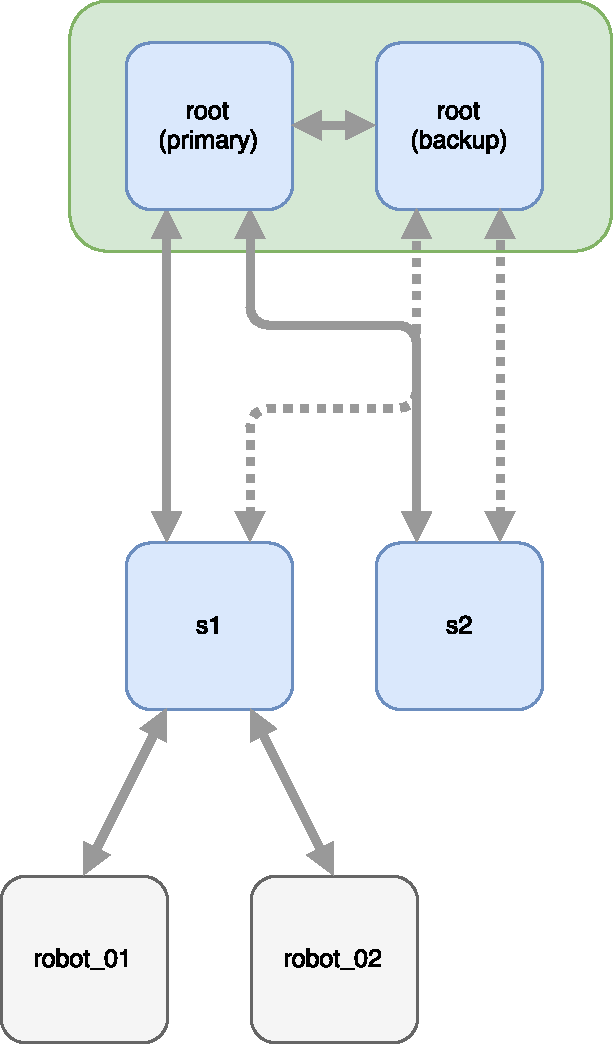
\includegraphics[width=0.4\textwidth]{img/logical_federation_setup.pdf}
	\caption{Logical federation topology used in system tests.}
	\label{fig:testing:topo:logic}
\end{figure}

As per \autoref{fig:testing:topo:logic}, the root node is a HA cluster, which
acts as such when appropriate according to
the feature being tested. At other times, only its primary node is active and
thus acts as a non-HA supernode of sN1 and sN2. The naming scheme is enforced
by Mininet and thus somehow clunky and cryptic.

The configuration also dictates that there are two simulated robots running on
subnode sN1, which continually update sensor data in the DIM and create new
cases due to their nature of virtually moving around randomly and thus trying
to escape the bounding box.

Subnode sN2 merely acts as a listener and is not directly supervising any field
devices.

\subsubsection{Virtual network plan}
\begin{figure}[]
	\center
	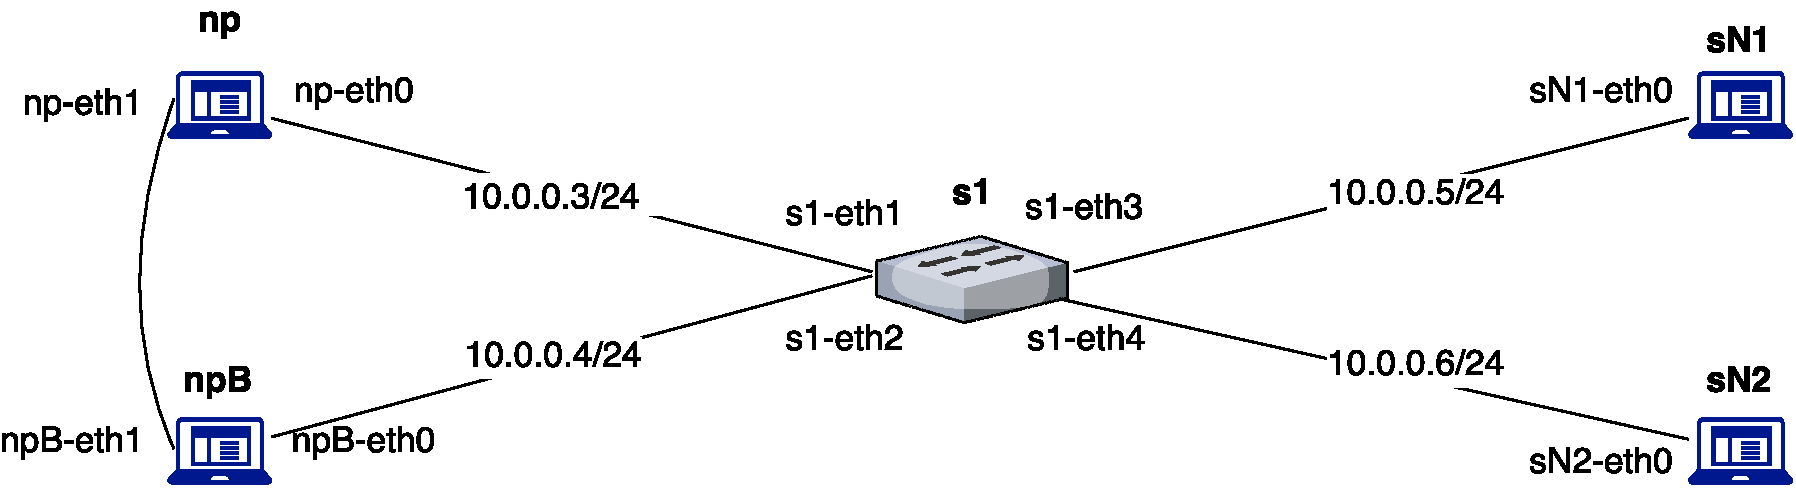
\includegraphics[width=\textwidth]{img/physical_network_mininet.pdf}
	\caption{Physical federation topology used in system tests.}
	\label{fig:testing:topo:physical}
\end{figure}

\autoref{fig:testing:topo:physical} illustrates the virtual network plan used in the system tests.
All nodes are attached to an \gls{ovs} instance which allows them communicate with each
other via the TCP/IP transport. In addition to this star topology, there is an
additional, dedicated link between the two HA peers which form the root HA
cluster.

% TODO how to test persistence synchronization
\subsubsection{Feature tests in detail}
In general all feature tests directly monitor the console output of each roadster instance.
The output is observed using different regular expressions to verify the behavior is correct.

In order to test persistence synchronization not only the Roadster console output is captured, 
but also the files are monitored for modifications. This ensures that the requested data
are persisted.

\paragraph{Encrypted network traffic}
To verify that the inter-node traffic is encrypted, it is captured too. The entropy is then calculated
based on that traffic dump of the exchanged messages. The minimum for the entropy efficency is set
above 95\%. It does not approach 100\% because \gls{ZMTP} control
commands are sent unencrypted, as defined in \cite[High-level
Grammar]{zmq:curvezmq}.

The entropy efficiency is defined as $\eta(X)$ as follows, which has been
implemented as part of the system test suites:

\begin{center}
$\eta(X) = -\sum_{i=1}^n \frac{p(x_i) \log_b (p(x_i))}{\log_b (n)}$,
\end{center}

where $p(x_i)$ is the probability of a certain character (the byte $x_i$)
within the encrypted traffic $X$, and $n$ is the cardinality of the chosen
script, which are all 256 possible values of one octet. More about the exact
approach to implement encryption in \autoref{sec:approach:encryption}.

Measurements have shown (\autoref{lst:ent:plain}) that the information
efficiency of unencrypted network traffic of Roadster amounts to $\sim$67\%.
The \sh{ent} tool has been used to perform this measurement before implementing
the calculation in the system tests themselves to reduce external depenencies.

\begin{listing}
	\begin{minted}[bgcolor=bg]{Text}
Entropy = 5.390141 bits per byte.

Optimum compression would reduce the size
of this 4518 byte file by 32 percent.

Chi square distribution for 4518 samples is 36298.08, and randomly
would exceed this value less than 0.01 percent of the times.

Arithmetic mean value of data bytes is 83.2517 (127.5 = random).
Monte Carlo value for Pi is 4.000000000 (error 27.32 percent).
Serial correlation coefficient is 0.310227 (totally uncorrelated = 0.0).
	\end{minted}
	\caption{Entropy statistics of plaintext network traffic.}
	\label{lst:ent:plain}
\end{listing}


%----------------------------------------------------------------------------

\clearpage
\section{Port to new \zmq binding}\label{sec:approach:port}
One of the first changes to Roadster's codebase is porting to a new \zmq
binding. This makes sense for the following reasons:

\begin{itemize}
\item To exclude possible failures from faults in the unmaintained ffi-rzmq\footnote{\url{https://github.com/chuckremes/ffi-rzmq}} library.
\item Encryption is needed later anyway, which is not supported by the currently used library.
\item All other tasks involve \zmq communication anyway.
\end{itemize}

There is currently only a single Ruby package that is maintained, supports
encryption, and is freely available, which is \gls{cztop}. Technically it is a
binding for the \gls{czmq} abstraction library, which is the modern and recommended way of
using \zmq. \autoref{sec:zmq:czmq} explains CZMQ in further detail.

As stated in the task description already, Roadster's event loop makes use of
the \zmq options \sh{ZMQ_FD} and \sh{ZMQ_EVENTS}. These are necessary to get a
file descriptor for each \zmq socket, which is then registered in the
Eventmachine reactor loop to be watched for readability. The second option is
then needed to actually confirm the situation of pending messages, since
readability of the file descriptor does not necessarily mean that a complete message
is available for reading yet. Getters for these two options had to be
added to in CZTop, which was a matter of minutes.

Due to Roadster's software architecture where different concerns
are cleanly separated, all code that actually depended
on ffi-rzmq was located in a single file. The following
things needed to be done:

\begin{itemize}
\item Load CZTop instead of ffi-rzmq.
\item Remove code to manually send and receive the parts of multi-part messages. This has been simplified
in CZMQ and thus is now a single method call.
\item Remove error checking code. CZTop always checks error codes, and raises
an appropriate exception if needed. These exceptions are now translated to Roadster's internal exceptions.
\item Simplify code that deals with \zmq options such as \sh{ZMQ_FD} and \sh{ZMQ_EVENTS}.
\item Replace library calls to use CZTop instead of ffi-rzmq.
\end{itemize}

This was about an hour's work.


%----------------------------------------------------------------------------
\clearpage
\section{Federation}\label{sec:approach:federation}
Running multiple Roadster nodes can be useful to aggregate information from
several field devices, especially if they cannot be connected to the same node,
possibly because of physical distance. Such a federation of autonomously
running nodes can then aggregate information in the root node, which can then
provide it to higher level client systems. Also, the root node's web UI shall
serve as a centralized point of access to the federation and offer an overview
of it to operational and technical personnel.

A Roadster federation consisting of a root node and two subnodes is illustrated
in \autoref{fig:federation}.
\begin{figure}[]
	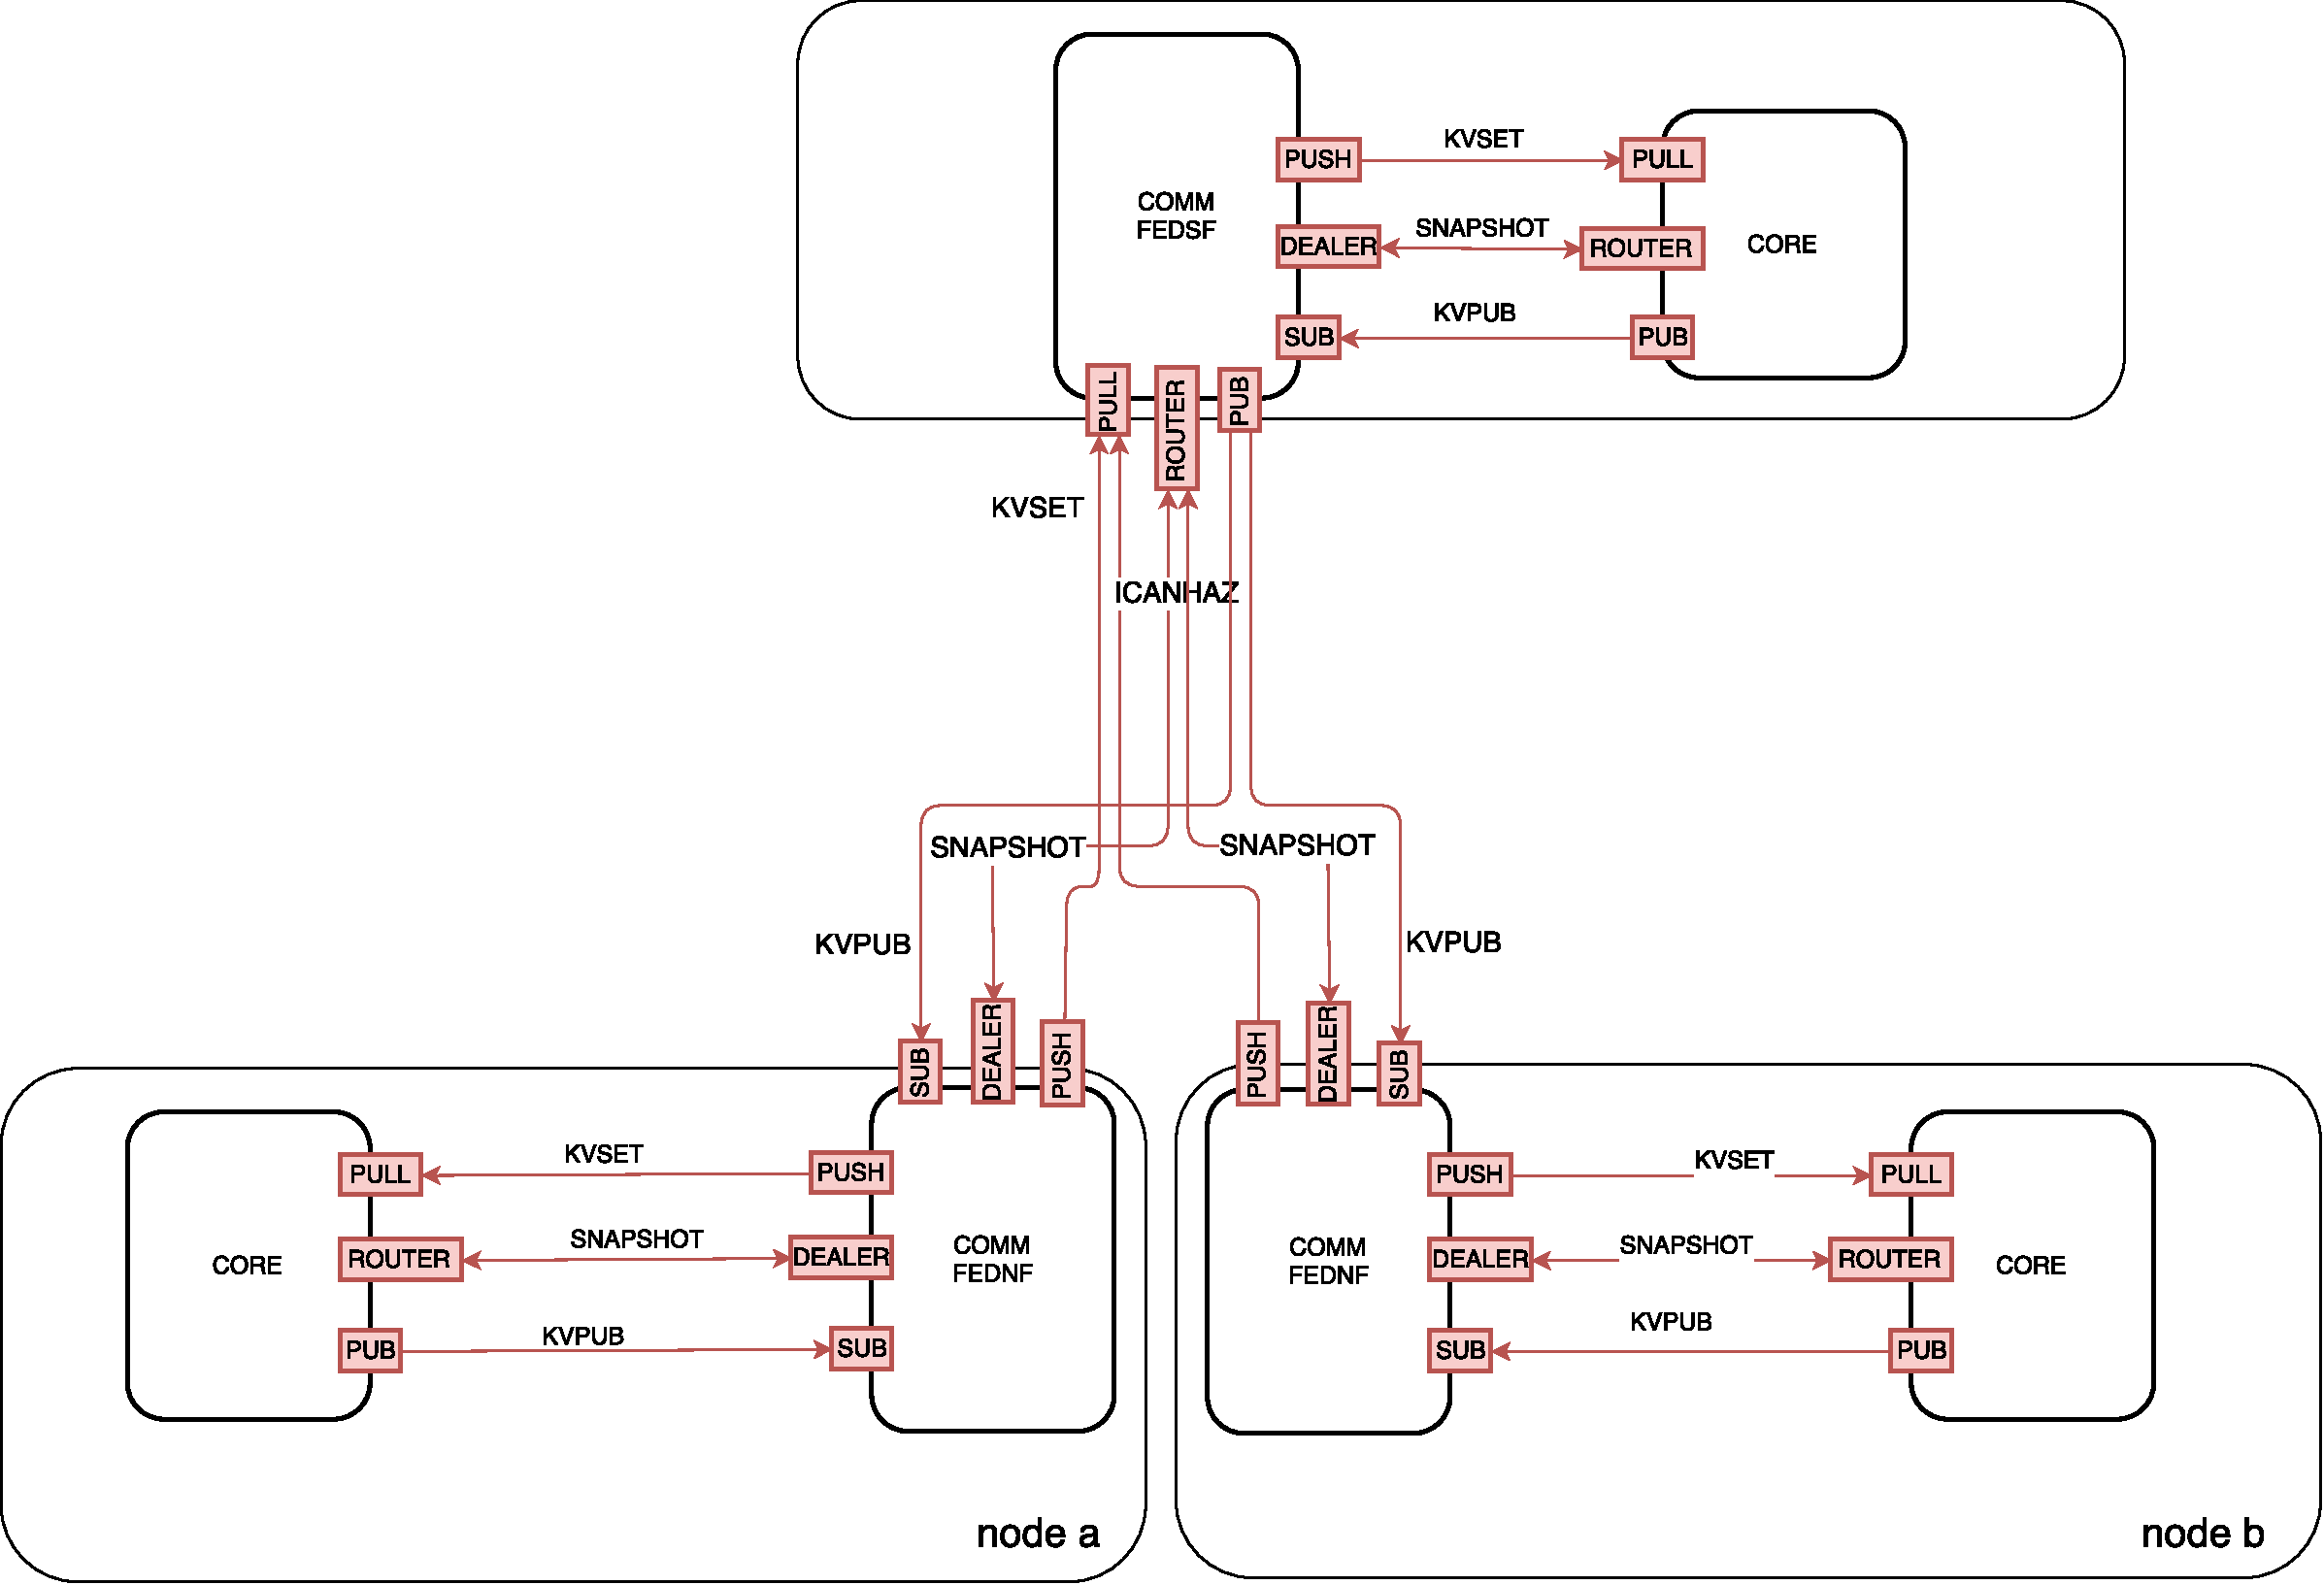
\includegraphics[width=\textwidth]{img/federation_protocol.pdf}
	\caption{Federation between a supernode and two subnodes.}
	\label{fig:federation}
\end{figure}

Adding federation functionality to Roadster involves the following aspects:
\begin{itemize}
	\item Means to declare a federation
	\item Message routing
	\item Heartbeating
	\item Inter-node CSP
	\item Remote alarm case management
\end{itemize}

\subsection{Federation declaration}
The federation topology has to be declared somewhere. This can be done using a
\gls{DSL} and then put into a static file shared
on all nodes of a Roadster federation. Each actor could then read the file at
startup, just like it is done for other configuration pieces of a Roadster node.

\autoref{lst:dsl:topo:no-ha} shows how such a configuration might look.

To allow the actors of a node to deduce which node they belong to, it is
necessary to provide an additional configuration, e.g. \sh{conf.local_node}.
This option then can be set in the node-specific configuration file as shown in
\autoref{lst:conf:root}.

\begin{listing}
	\begin{minted}[bgcolor=bg]{Ruby}
# Roadster application configuration
module Roadster

  conf.local_node = 'root'

  conf.log_level = ::Logger::Severity::INFO
  conf.pid_file  = File.join conf.root, 'log', 'root.pid'
  conf.log_file  = File.join conf.root, 'log', 'root.log'
  conf.data_path = File.join conf.root, 'data.root'

  conf.webserver_port = 3010
  conf.environment = :development
end
	\end{minted}
	\caption{Node-specific configuration of the node 'root'.}
	\label{lst:conf:root}
\end{listing}

Not every node in a federation is the same: Each one has its own set of field devices (if any).
The configured name of the local node can be used in conjunction with the
federation topology declaration to deduce important information such as neighboring
nodes and the exact set of adapters to load on the local node.

\begin{listing}
	\begin{minted}[bgcolor=bg]{Ruby}
module Conf::Federation
  def self.conf
    proc do
      primary_endpoints \
        router: 'tcp://0.0.0.0:20000',
        pull:   'tcp://0.0.0.0:20001',
        pub:    'tcp://0.0.0.0:20002'

      adapters do
        adapter :foobar do
          # config for 'foobar' adapter and its peers
        end
      end

      node :s1 do
        adapters do |s1_node|

          adapter :simu do
            label           'SIMU'
            desc            'Process simulation adapter'
            adapter_class   Roadster::Adapters::Simulation

            peer :robot_controller_01 do
              label 'robot_01'
              uri   ''
            end

            peer :robot_controller_02 do
              label 'robot_02'
              uri   ''
            end
          end
        end

        objects do |s1_node|
          robot :robot_01 do
            label_i18n  de: 'Mein schicker roboter nummer 1',
                        en: 'My fancy robot number 1'
          end
          s1_node.objects.robot_01.reference_peer s1_node.adapters.simu.robot_controller_01

          robot :robot_02 do
            label_i18n  de: 'Mein schicker roboter nummer 2',
                        en: 'My fancy robot number 2'
          end
          s1_node.objects.robot_02.reference_peer s1_node.adapters.simu.robot_controller_02
        end
      end
    end
  end
end
	\end{minted}
	\caption{Federation DSL example without HA.}
	\label{lst:dsl:topo:no-ha}
\end{listing}


\subsubsection{Inter-node sockets}
To provide all functionality used by any of Roadster's messaging protocols, the
new actors from the prototype are completed according to the illustration in
\autoref{fig:federation}. As a result, the COMM.DOWNSTREAM actor registers a
ROUTER, a PULL, and a PUB socket, whereas the COMM.UPSTREAM actor registers a
DEALER, a PUSH, and a SUB socket.

\subsection{Message routing}\label{sec:approach:msg-routing}
Messages need to be sent from an actor on one node to an actor on another node.
The best place to put this logic is the CORE actor which already does this for
messages exchanged within a node. The existing mechanism needs to be extended to take other nodes
into consideration as well. Then messages can be passed around hop-by-hop.

Message routing shall be stateless, following the well-known and battle proved
example of routing in \gls{IP}. This means that even a message sent in
\emph{Dialog} mode shall not leave pending resources acquired on nodes other
than the source and the destination node.


The \sh{Roadster::Messaging::Messages::Base} class has been extended to accept
not only a destination actor as recipient, but also a node. The simplest way
possible, which also happens to be very convenient when writing protocol code,
is to follow the email example, e.g. \sh{actor@node}. The \sh{node} is actually
the full path of a node, starting from the root node. As an example, a message
sent to the CORE actor of the node \sh{root.s1}, the recipient shall be
\sh{core@root.s1}.

If the recipient node is not specified, the local node shall be inserted
automatically upon sending. The same applies to the source node. This is to
ensure that legacy code unaware of the federation feature still works as expected.

Any message that is to be routed shall be sent to the CORE first, which was
already the case before this bachelor thesis. What the CORE now does, is
inspect the message's recipient: If it's destined to the local node, it is
handled as always. Only if the destination node is a remote node, the new
routing logic in \sh{Roadster::Messaging::FCP::Core} comes into action.

Routing within a hierarchical topology is very easy, especially when the
recipient's full path within the hierarchy is part of the message. If the
recipient node's path is not a prefix of the local node, the next hop has to be
the supernode. Otherwise, it has to be one of the subnodes, which is determined easily,
being simply the path one component longer than the one of the local node.

Due to the hierarchical property of Roadster federations, network loops are
definitely not present. This simplifies the routing mechanism further, because
no means of limiting a message's lifetime is necessary, as it is in \gls{IP} in
the form of a time-to-live field. IP needs this mechanisms because network
topologies can change at any time, even creating loops, which could then result
in a packet circulating indefinitely.

Any wrong recipient set in the message results in the message being discarded
immediately by the ROUTER socket if it is not aware of a corresponding remote socket.

 The complete code for this routing algorithm is illustrated in
 \autoref{lst:approach:msg-routing}.


\begin{listing}[H]
	\begin{minted}[bgcolor=bg]{Ruby}
class Core < BaseAPI
  def initialize(messaging)
    super
    @subnode_regex = /^#{Regexp.escape local_node}\.\w+/
    @supernode = local_node.split('.')[ 0 .. -2 ].join('.')
  end

  # Forward message using messaging layer. Either to local actor or to
  # remote node.
  #
  def forward_message(msg)
    if local_node == msg.receiver_node
      # local delivery
      msg.add_envelope msg.receiver
    else
      set_next_hop msg
    end

    messaging.forward_message msg
  end

  private

  # Lookup and set next hop(s) of message using "string based"                                                                                                             # routing. It's either forwarded to the supernode or one of the
  # subnodes.                                                                                                                                                              #
  # @param msg [Messaging::Messages::Base] the message to prepare for                                                                                                      #   the next two hops to another node
  #                                                                                                                                                                        def set_next_hop(msg)                                                                                                                                                      if subnode = msg.receiver_node[ @subnode_regex ]
      # forward to/via subnode
      msg.add_envelope "comm.upstream@#{subnode}"      # second hop
      msg.add_envelope "comm.downstream@#{local_node}" # first hop
    else
      # forward to/via supernode
      msg.add_envelope "comm.downstream@#{@supernode}" # second hop
      msg.add_envelope "comm.upstream@#{local_node}"   # first hop
    end
  end
end
	\end{minted}
	\caption{Message routing algorithm.}
	\label{lst:approach:msg-routing}
\end{listing}


\subsubsection{Example}
When a user of the root node's web UI wants to change a value on a field device
connected to the root node's subnode, a command is sent from the browser to the
root node's COMM.WEBUI actor. From there it is sent to the CORE actor, which
routes it via the DOWNSTREAM actor to the subnode. There it is relayed by the
COMM.UPSTREAM actor to the the CORE actor, which then routes it locally to the
correct COMM actor, which in turn executes the command on on the field device.


\subsection{Heartbeating}\label{sec:approach:hb}
To avoid filling a PUSH socket in case the supernode is unavailable, and also
just to keep an up-to-date view of neighboring node's liveliness, heartbeating
is performed between a supernode and its subnodes.


Two new message types have been defined:
\begin{itemize}
	\item \sh{Roadster::Messaging::FCP::Messages::Ping}
	\item \sh{Roadster::Messaging::FCP::Messages::Pong}
\end{itemize}

Two-way heartbeating (ping/pong) is used, where the supernode periodically
sends a Ping message to all its direct
subnodes. This is done via the COMM.DOWNSTREAM's PUB socket (one-to-many).
Every subnode then replies with a Pong
message, done via the COMM.UPSTREAM's DEALER socket (one-to-one).

Each received Pong message proves to the supernode that the respective subnode
is responsive. Of course, this also applies to the Ping message: Receiving a
Ping message tells the subnode that its supernode is responsive.

The implementation actually sends a sequence number with every Ping message,
which is then echoed as part of the Pong message. This makes it possible to
recognize the situation of a much delayed Pong message, including the
calculation of the exact delay (spanning multiple Ping periods).

Why are Pings not sent in the \emph{Dialog} mode? Dialog messages are not
suitable for one-to-many communications.

The \gls{ZMTP} version 3.1, as supported by recent versions of \zmq, actually
contains a heartbeating feature. But ZMTP 3.1 is not stable yet as of this
writing, and in case a remote socket becomes unresponsive, the connection is
silently disconnected, which is not very useful to keep track of neighboring
nodes' liveliness. Its intended use is to detect stale TCP connections and thus
release possibly blocked processes.

For the aforementioned reasons, application heartbeating is performed.

Due to the message routing being used for the Pong message, a full cycle of
Ping/Pong involves the following actors, starting with the Ping message being
published via the inter-node PUB socket:
\begin{enumerate}
	\item COMM.DOWNSTREAM of the supernode
	\item COMM.UPSTREAM  of the subnode
	\item COMM.CORE of the subnode
	\item COMM.UPSTREAM of the subnode
	\item COMM.DOWNSTREAM of the supernode
	\item COMM.CORE of the supernode
	\item COMM.DOWNSTREAM of the supernode
\end{enumerate}

This is good because it means both CORE actors of any supernode-subnode pair
are involved. In case, for some reason, the CORE actor is unresponsive, Ping
messages are not simply echoed by the COMM.UPSTREAM actor, which is the desired
behavior.


\clearpage
\subsection{Inter-node CSP}
The DIM has to be replicated across a hierarchical federation of nodes, as the
DIM is the essential data structure representing the overall state of a
Roadster federation.

One of the new actors' responsibility is the replication of updates to the DIM,
similar to how the \gls{CSP} works within a single node.  To do so, both the
COMM.UPSTREAM and COMM.DOWNSTREAM actor simply subscribe to DIM updates within
a node just like any other COMM actor does.  Then they replicate any subsequent
updates over the network to the neighboring nodes. The existing three socket
pairs are used, since they are protocol agnostic thanks to Roadster's layered
architecture.

\paragraph{Replication is bidirectional}
It is possible that two sibling nodes will have performed modifications to the
DIM while they were disconnected from their common supernode. Thus, the initial
exchange of snapshots, as well as the subsequent propagation of modifications
to the DIM has to be bidirectional.

\paragraph{CAP theorem}
The CAP theorem \cite{wp:cap} states that it is impossible for a distributed
computer system to simultaneously provide consistency, availability, and
network partition tolerance. In the face of a network partition, one has to
chose between availability and consistency. Because subsystems of a Roadster
federation must be autonomous, the obvious choice is availability. Eventual
consistency is achieved when recovering from a network partition by simply
reinitiating the DIM replication process.


\subsubsection{Degree of replication}
There are several variants when it comes to how much exactly of the DIM should be replicated:
\paragraph{Variant 1: Self-subtree only}
Synchronize on subtree only, which means a node only knows the DIM part of
itself. The big disadvantage is that it will not have a copy of the rest of the
DIM, which can be useful to inspect variables on neighboring nodes, especially
when they're unreachable.

Note that this would only work because of the rearrangement of DIM objects
described in \autoref{sec:approach:dim:ownership}. Otherwise the objects
belonging to a single node would reside within separate subtrees.

\paragraph{Variant 2: Complete tree}\label{par:approach:dim:var2}
Always synchronize on complete tree, which means getting the snapshot from the
supernode and merge the own subtree into it, replacing whatever subtree is
already there. This works because of the autonomy requirement for nodes and
their subnodes. This variant is very easy to implement at first.

\paragraph{Variant 3: Either subtree or complete tree}
Make it configurable: Either synchronize on the subtree or on complete tree. The
topology DSL could allow specifying this as a property for each node. This is
the best of both worlds, but more effort.

Variant 2 will be the first step, as following the \gls{KISS} principle is one
of the non-functional requirements. Variant 3 will be the second step, if at
all. This depends on whether it will be necessary, e.g. if replicating the
total DIM is feasible performance-wise.

\subsubsection{Ignoring update reflections}
Because of the way the \gls{CSP} works, modifications to the \gls{DIM} pushed
to the supernode have to be published back to all subnodes, just like the CORE
actor publishes modifications to back to all local actors. That means the update is
also reflected back to the subnode on which the update originated. A subnode's
UPSTREAM actor has to recognize this situation and discard the update in question
immediately.

This is easily achieved by comparing the version number, because a reflected
update always has a version number $\leqslant$ the local version number.


\subsubsection{Object ownership}\label{sec:approach:dim:ownership}
The concept of ownership has to be introduced. Every object within the DIM
shall belong to a particular node. Modifications to the objects shall be done via
that node, and only that node, so the node is the authorative instance for all modifications of its own objects.
For that, every object in the DIM has to have a reference
to the object representing its owner node, which is part of
the configuration that is loaded from the static configuration loaded by every
actor at initialization.

Some objects like parameters (described in \autoref{sec:scope:persistence})
will apply to a whole federation and will thus be owned by the root node.
Examples of these are UI user credentials.

To avoid having to store an additional reference to a node object in every DIM
object, the process of finding its owning node can be simplified by rearranging
the objects. Making all objects direct or indirect children of the owning node
means that determining their owning node is merely a traversing of the tree up
to the first node object.

As a result, the existing domain model class \sh{Roadster::Domain::Model::Root}
has been eliminated. Instead, the root node's
\sh{Roadster::Domain::Model::Node} object takes its place in the DIM. As a
consequence, the whole configuration of adapters, field devices, aggregates,
and such now belong to the root node. Of course, the same goes for any subnodes
and their configuration.

\subsubsection{Write access control}
% TODO: DIM access control
The class \sh{Roadster::Domain::Host} provides functionality around accessing
and traversing DIM objects. A few existing, cohesive methods in it used to
apply model updates have been refactored and extracted into a new class
\sh{Roadster::Domain::Host::ModelUpdater}.

This new class also enforces write access control, which is new functionality.
All updates to objects owned by the local node (except version numbers) must
originate from the local node. Updates affecting foreign objects are allowed by
any node. Further access control checks are not performed, since the updates
could traverse several nodes before reaching the local node.

% NOTE: This is a different kind of access control:
%Each node has its own access control. Only roles and user data are obtained 
%from the root node.


\subsubsection{Version monotonizing}
In case a node has to be rebooted due to whatever reason, its version numbers
start over at zero.
This leads to the situation where its domain model updates sent to neighboring
nodes are discarded as being outdated, until they reach their previous value.
This is why snapshots from neighboring nodes are initially requested to
instantly increase the version numbers to their previous value.

The implementation is straight-forward. When applaying a snapshot --- as well as regular
updates --- a mere monotonical increase of the version number is enforced by
taking the maximum of the two, no matter if the increase was caused by local or
an foreign snapshot.

\paragraph{Bootstrapping}
When starting an entire federation of nodes, and each node initializes foreign
node versions to zero, the very first update or snapshot from that node would
be recognized as outdated and thus discarded. This is why all
\sh{Roadster::Domain::Model::Node} instances representing foreign nodes are
initialized to version -1, so the very first update ($\geqslant 0$) is always
applied.
% TODO: supernode implementation braucht dieses Funktion auch - weil

\subsubsection{Shared functionality}
The \gls{CSP} has to work as an intra-node protocol (within a node, which is
the legacy behavior), as well as an inter-node protocol (within a federation).
That means \gls{CSP}-related server functionality has to be present in the CORE
engine, as well as in the DOWNSTREAM engine. CSP-related client functionality has
to be present in all existing COMM engines, the UPSTREAM engine, \emph{as well
as the DOWNSTREAM engine}, since it also acts as a CSP client to the CORE engine on
the same node.

To avoid a considerable amount of code duplication, CSP-related functionality
has been extracted into its own reusable module \sh{Roadster::Engines::CSPMethods}, which is then mixed into all
relevant actors. The \emph{Template Method} design pattern is used to handle
the common case of handling a received
\sh{Roadster::Messaging::CSP::Messages::ModelUpdate} message. The hook methods,
called by the template method, are then implemented
in each particular class where necessary. Where no special behvior is needed,
the mixed-in methods are left unchanged.

\subsubsection{Summary}
\autoref{fig:csp:upstream-activity} and \autoref{fig:csp:downstream-activity}
are the exact activity diagrams for the COMM.UPSTREAM and COMM.DOWNSTREAM
actors, respectively.

A sequence diagram showing the replication process from an update from a
simulated field device across a supernode to another subnode is illustrated in
\autoref{fig:csp:version-sequence}.

\begin{figure}[]
	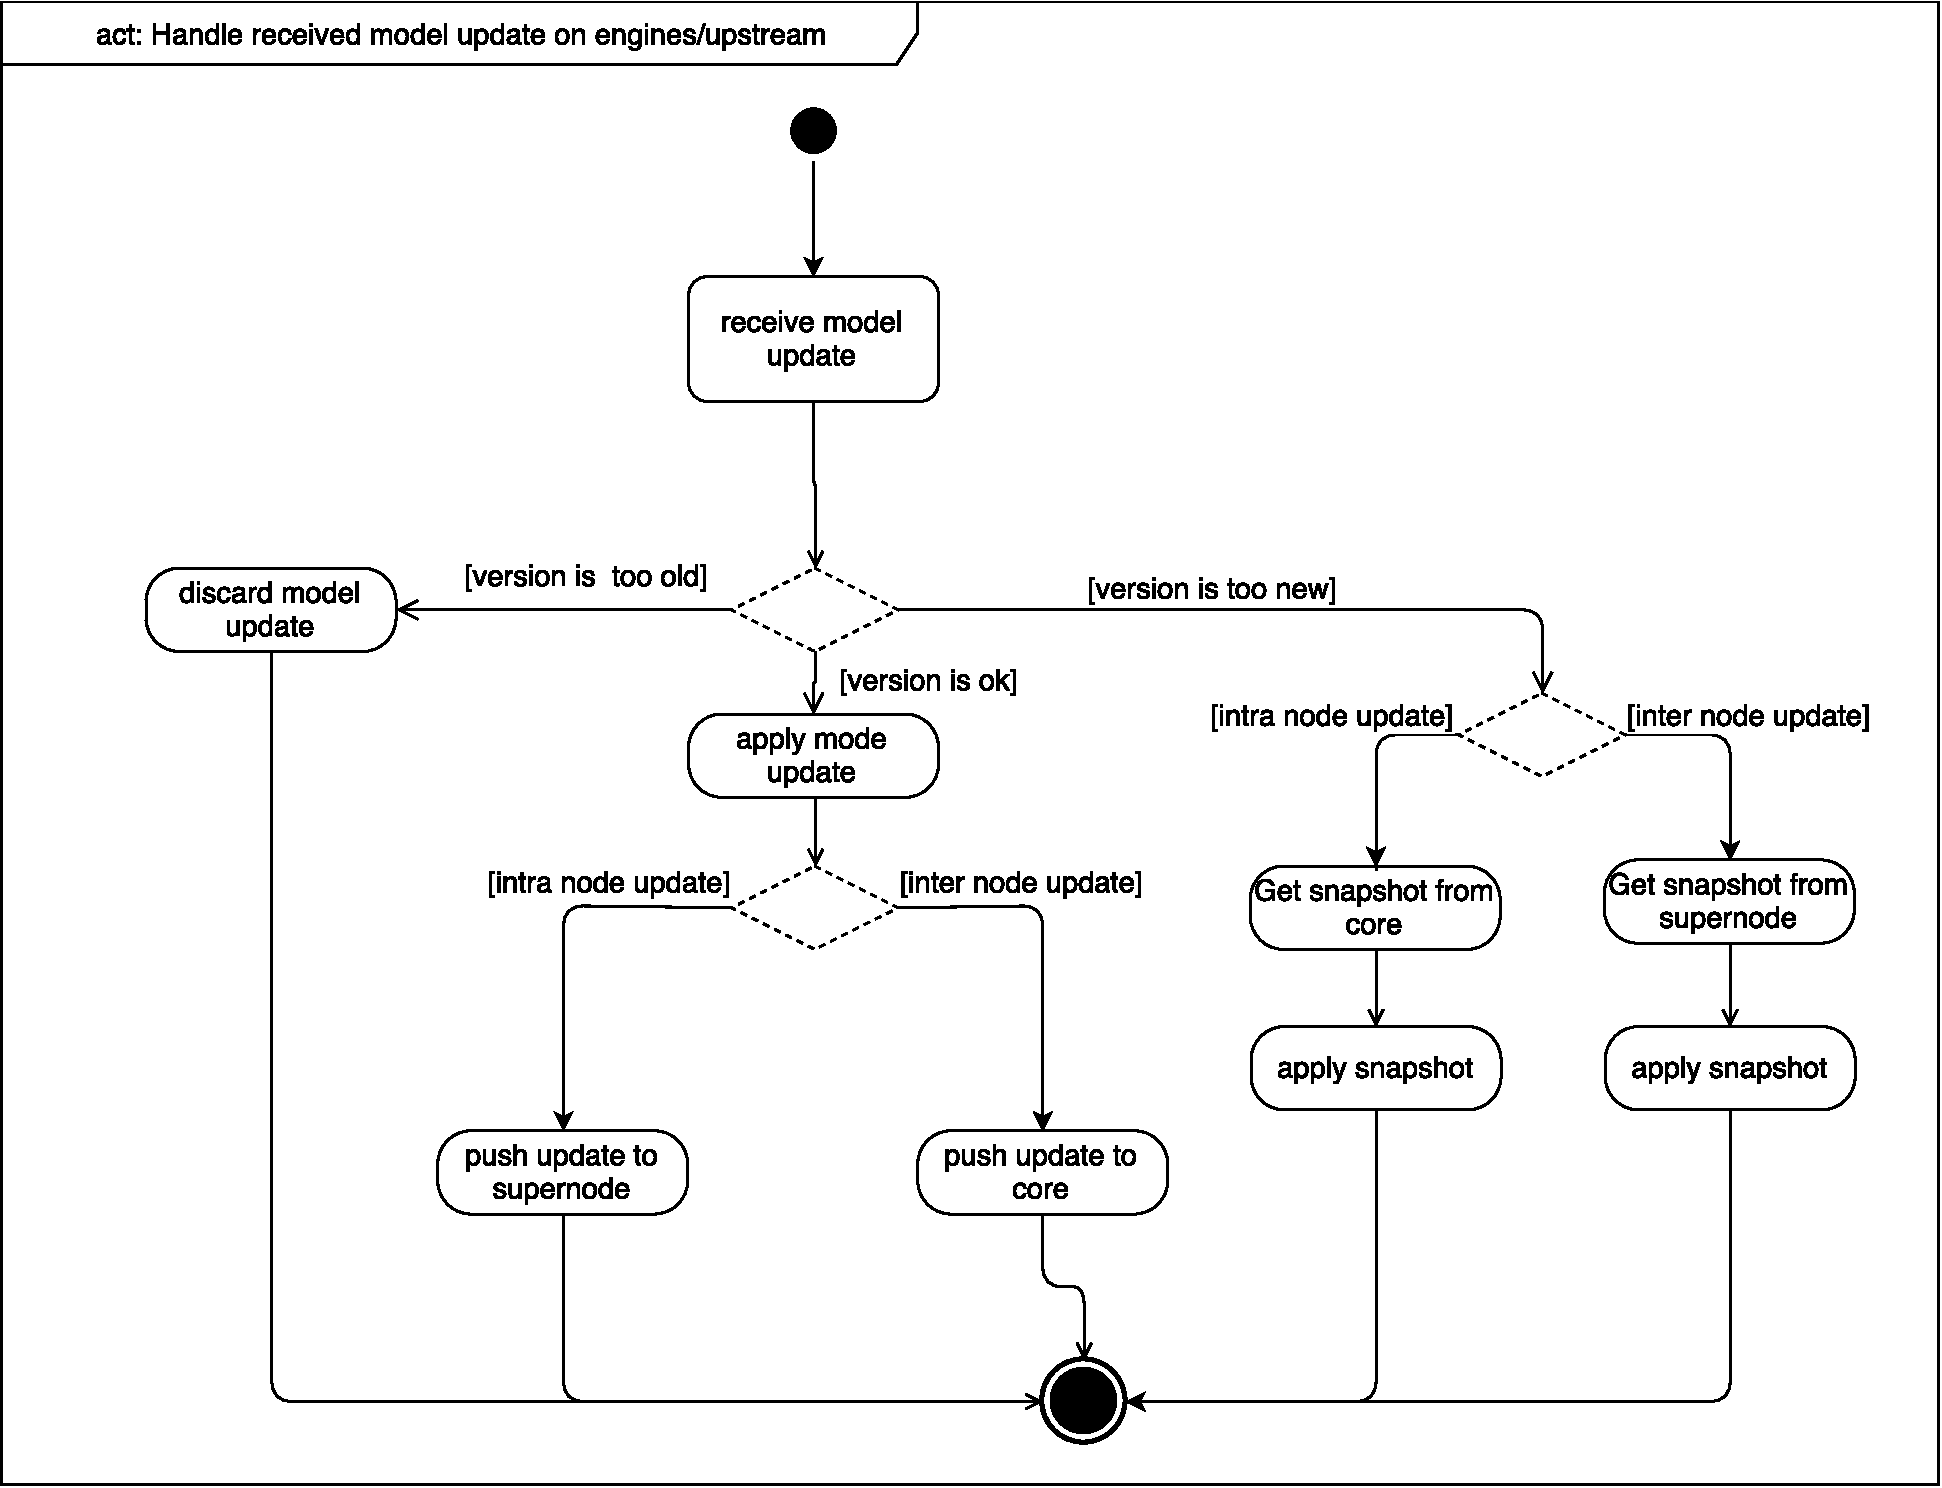
\includegraphics[width=\textwidth]{img/activity_diagram_upstream.pdf}
	\caption{CSP upstream activity diagram.}
	\label{fig:csp:upstream-activity}
\end{figure}

\begin{figure}[]
	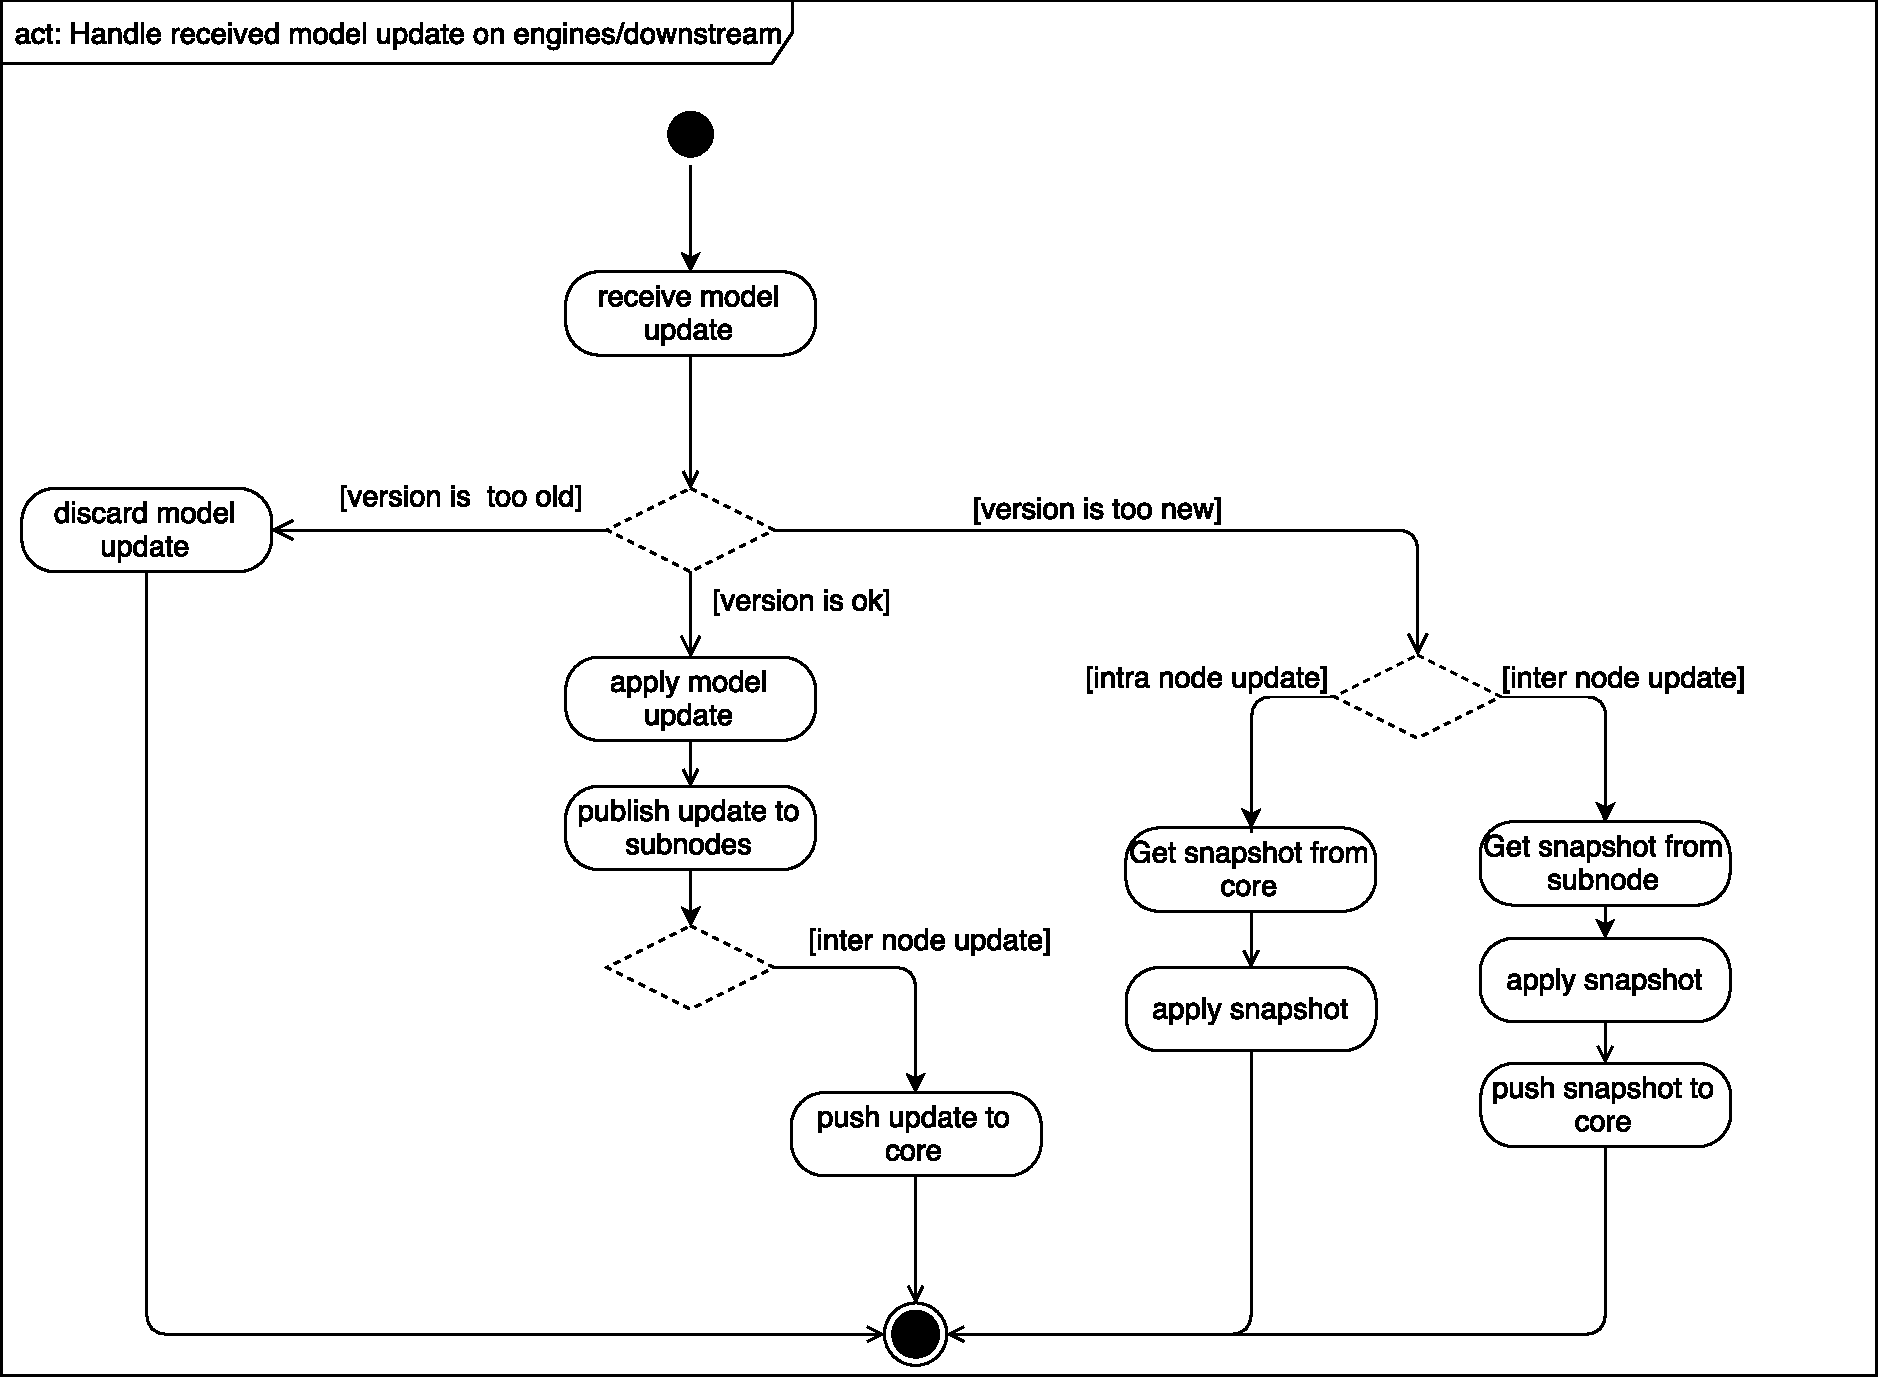
\includegraphics[width=\textwidth]{img/activity_diagram_downstream.pdf}
	\caption{CSP downstream activity diagram.}
	\label{fig:csp:downstream-activity}
\end{figure}

\begin{figure}[]
	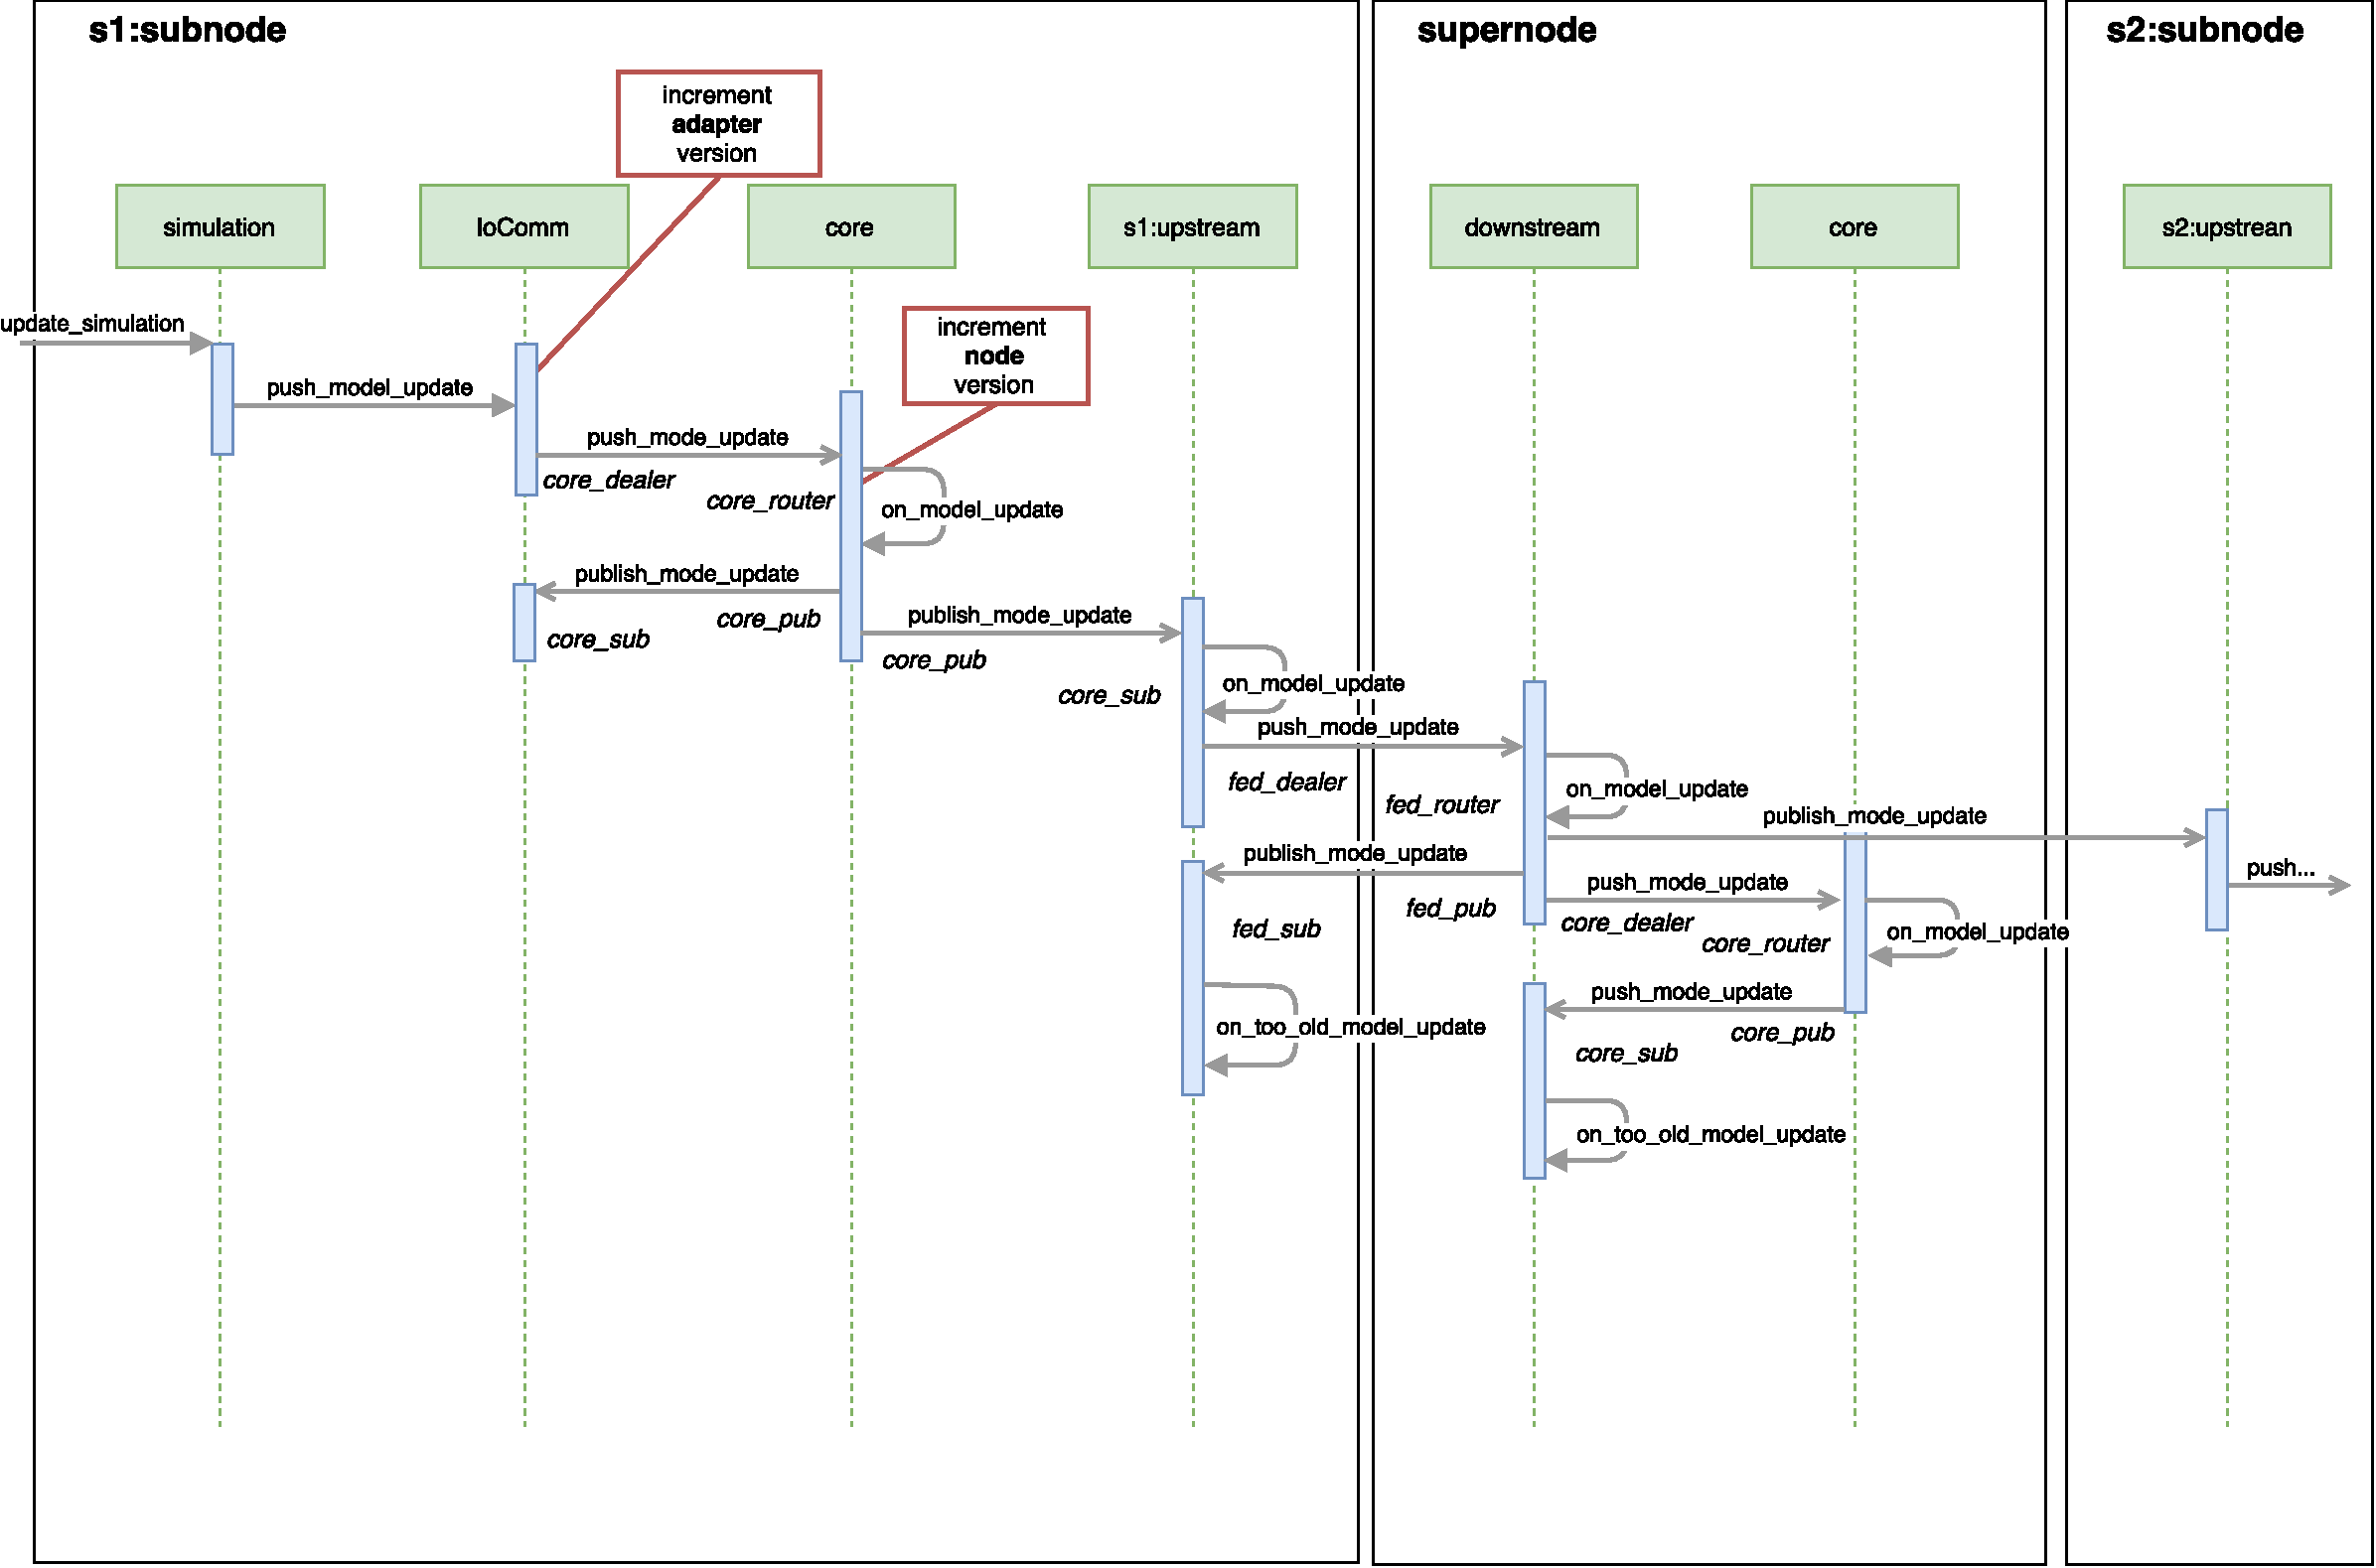
\includegraphics[width=\textwidth]{img/sequence_diagram_model_update_pub.pdf}
	\caption{CSP version sequence diagram.}
	\label{fig:csp:version-sequence}
\end{figure}




\subsection{Remote case management}
As defined by the access control restriction in the previous section, a case
can only be closed on the owning node of the case. Therefore, the command
for closeing the case must be sent to the owner node. To check the authorization
on the owner node, the sender node's ACL configuration --- part of the DIM --- is used, because only
the sender node has the appropriate session saved.
% TODO gem 'simple_states' failed and thus was dropped, reduced complexity
% TODO how to write your own FSM


%----------------------------------------------------------------------------
\clearpage
\section{High availability}\label{sec:approach:ha}
If Roadster is going to be run in a federation, measures need to be taken to
mitigate the risk of failure, since one in many nodes is more likely to fail than a
single node alone. This can be especially degrading to the service quality if
it is a common supernode, e.g. the root node in particular.

Availability shall be improved by adding redundancy on certain levels of the
node hierarchy in the form of a fully functional, running backup node in
addition to the primary one. Common usecases, as defined in \autoref{ch:reqs}
require that this works at least at the highest hierarchy level, i.e. the root
node.

Run together in a hot-standby cluster, the passive HA peer's responsibility is to
take over in case the active one fails to deliver its service.



\subsection{Defining reliability}
When speaking about reliability, it is worth listing the failures the solution must be
able to handle. According to the requirements, and thinking a bit further,
handleable failures of the following three categories have been identified:

\begin{description}
	\item [Hardware failure on the active HA peer:] \hfill\\
		No hardware runs forever. Any of the following things could
		happen spontaneously at any time:

		\begin{itemize}
			\item A non-redundant disk can fail fatally
			\item Memory can encounter an irrecoverable error
			\item The \gls{CPU} catches fire
			\item The node's power supply starts smoking
			\item The node's switch port can break
			\item The node's \gls{NIC} can break
			\item A power or network cable mysteriously fail due to wear and tear
			\item A random power outage that only affects one node
			\item Someone accidentally pulling the node's power
				plug or network cable (human-induced)
		\end{itemize}

	\item [Software failure on the active HA peer:] \hfill\\
		Bug-free software is rare, if it exists at all, and the
		following scenarios are possible:

		\begin{itemize}
			\item Roadster crashes, e.g. the CORE actor becomes unresponsive
			\item the disk becomes full
			\item the memory becomes full (and triggers the \gls{oom-killer})
			\item the whole OS freezes or crashes (less likely, but possible)
			\item Accidental shutdown of the currently active HA
				peer, either just the Roadster application, or
				the whole node (human-induced)
		\end{itemize}

		More about handling crashes of certain actors can be found in
		\autoref{sec:approach:ha:hb}.

	\item [Network failure:] \hfill\\
		This only includes:
		\begin{itemize}
			\item Failure of the link connecting a HA node to the
				rest of the federation.
			\item Configuration mistakes in
				switching/routing/firewall equipment which cut
				off the currently active HA peer (human-induced)
		\end{itemize}
\end{description}

Handling a failure means an actual service interruption can be avoided.

\subsubsection{Failures not handled}
Failures that do not have to be or cannot feasibly be handled include:

\begin{description}
	\item [Link failure between a subnodes and one of the HA peers:]\hfill\\

		This cannot be handled since the two HA peers would have to
		continually share the number of subnodes connected to them, and
		based on that, make a decision on which one should be active or
		passive. Since the link between them could fail as well, this
		decision cannot be done reliably, which could lead to the
		dreaded split brain syndrome.

		Actually the \gls{bstar} could be extended to support this kind
		of mechanism. The details are described in
		\autoref{sec:approach:ha:bstar-ext}.


	\item [Link failure between a HA peer and a field device:]\hfill\\
		The \gls{bstar} algorithm will not initiate a failover since the
		active peer is still responsive and is able to send heartbeats to the passive HA peer.

		The interrupted communication with the affected field device
		could and definitely should cause an alarm, but no failover,
		since they're only half of the conditions that have to be met
		for a failover.

		\autoref{sec:discussion:ha:manual-failover} describes a
		proposal for manually induced failovers.

	\item [ Complete network outage:]\hfill\\
		A complete network outage, such as caused by a routing or
		firewall configuration mistake, cannot be handled gracefully by
		Roadster.

	\item [ Non-redundant hardware failure:]\hfill\\
		In case non-redundant hardware fails, such as a whole network
		switch, cannot be handled gracefully by Roadster.

	\item [ Complete power outage:]\hfill\\
		A complete power outage will not be handled gracefully by
		Roadster. Providing a \gls{UPS} to keep Roadster nodes and
		network equipment up and running in such a case is matter of
		the respective facility in question.

	\item [ Natural disasters:]\hfill\\
		These cannot be handled gracefully by Roadster. Damage from an
		earth quake, a fire, meteorological disasters, solar flares, or
		similar, are outside of the scope of Roadster's high
		availability feature.
\end{description}

The \gls{zguide} describes a very simple mechanism to achieve this kind of high
availability with exactly two redundant nodes: The \gls{bstar}. It
provides a set of clients a highly available service by running two server
nodes in a hot-standby setup. It is simple and thus very robust, takes measures to avoid the
split-brain syndrome, and is fairly easy to implement, even as reusable
code.

The implementation could be contained within a new kind of COMM actor
called BSTAR. This makes sense since, in a way, it talks to the outside world.
That part of the outside world just happens to speak the same language. This
means that the new kind of actor most likely will not need an adapter like COMM
actors usually do in Roadster.

\subsection{Binary Star in a nutshell}
Two HA peers are started either as primary or as backup. After an initial
handshake, the primary one becomes active, the backup node becomes passive. The
two continually exchange their current state with regards to
the \gls{bstar}. This exchange also acts as heartbeating between the two HA
peers. The state machine of the \gls{bstar} is illustrated in the diagram
\autoref{fig:bstar:state}.

Clients and subnodes always connect to the primary HA peer's endpoints first. This
is illustrated in \autoref{fig:ml:ha}.

\begin{figure}[]
	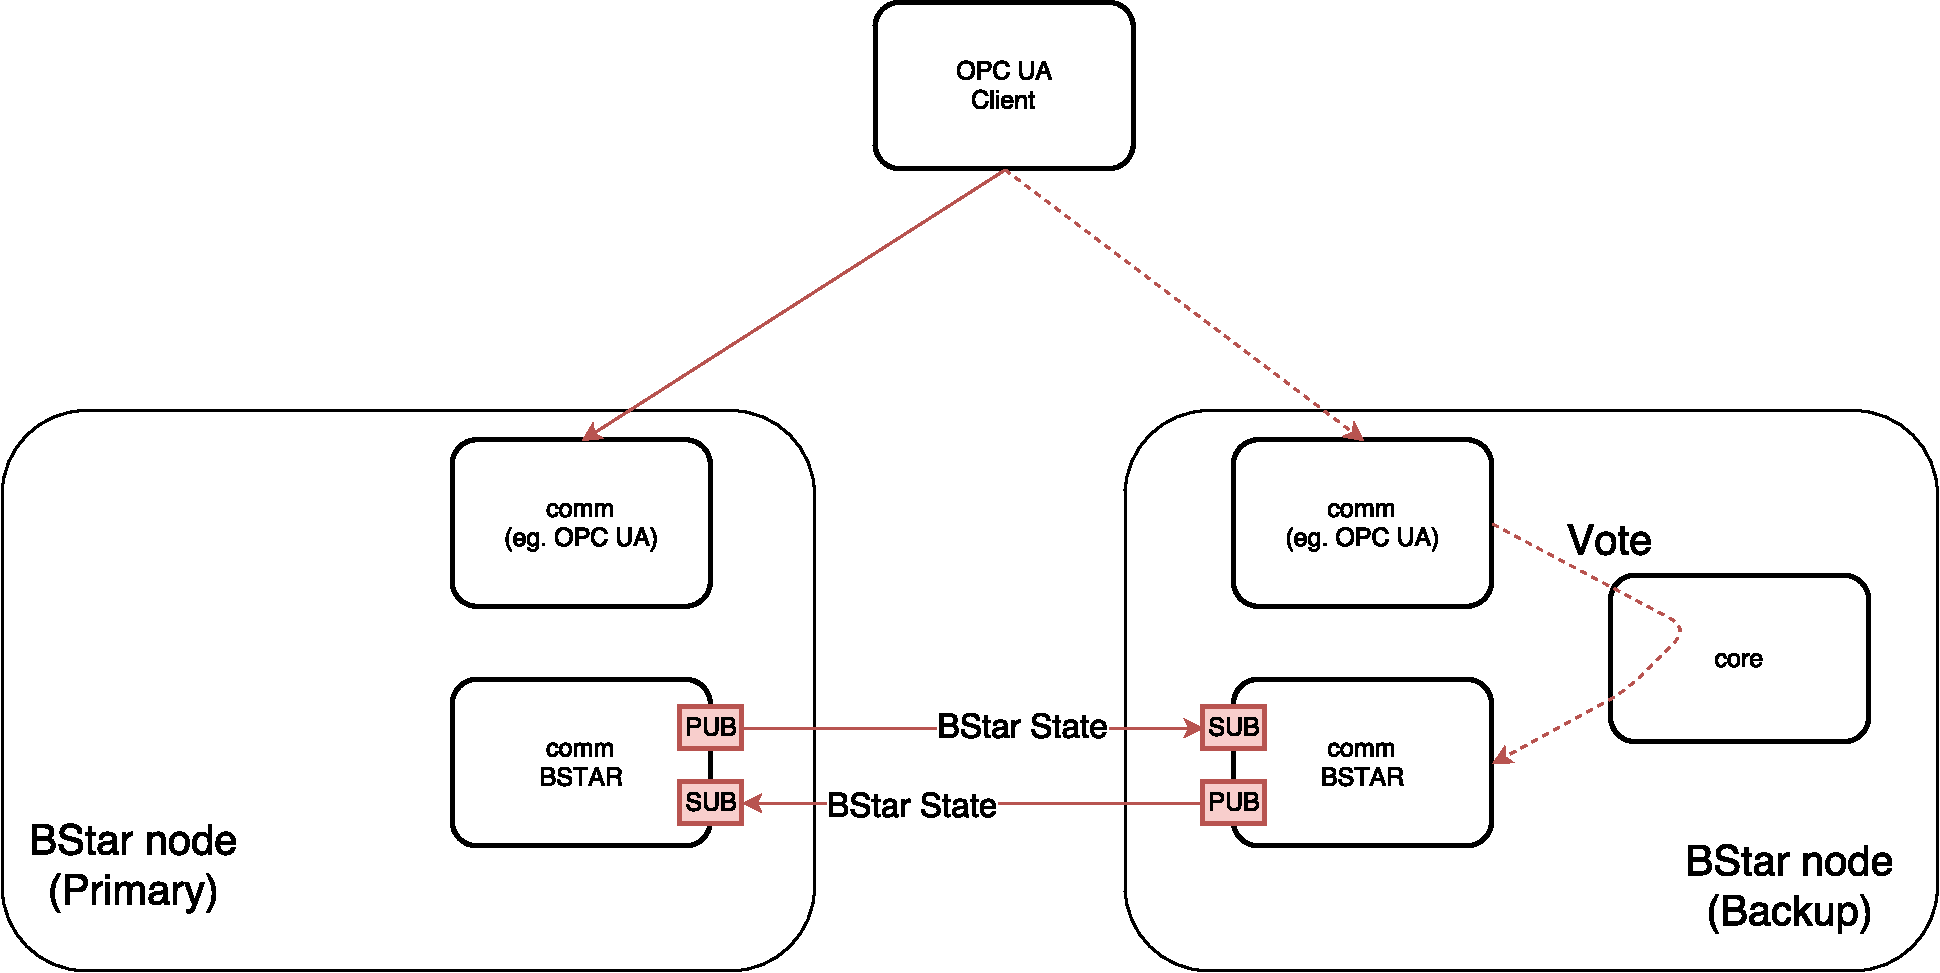
\includegraphics[width=\textwidth]{img/ML-HA_bstar.pdf}
	\caption{Schema of HA cluster and a higher level client.}
	\label{fig:ml:ha}
\end{figure}

\begin{figure}[]
	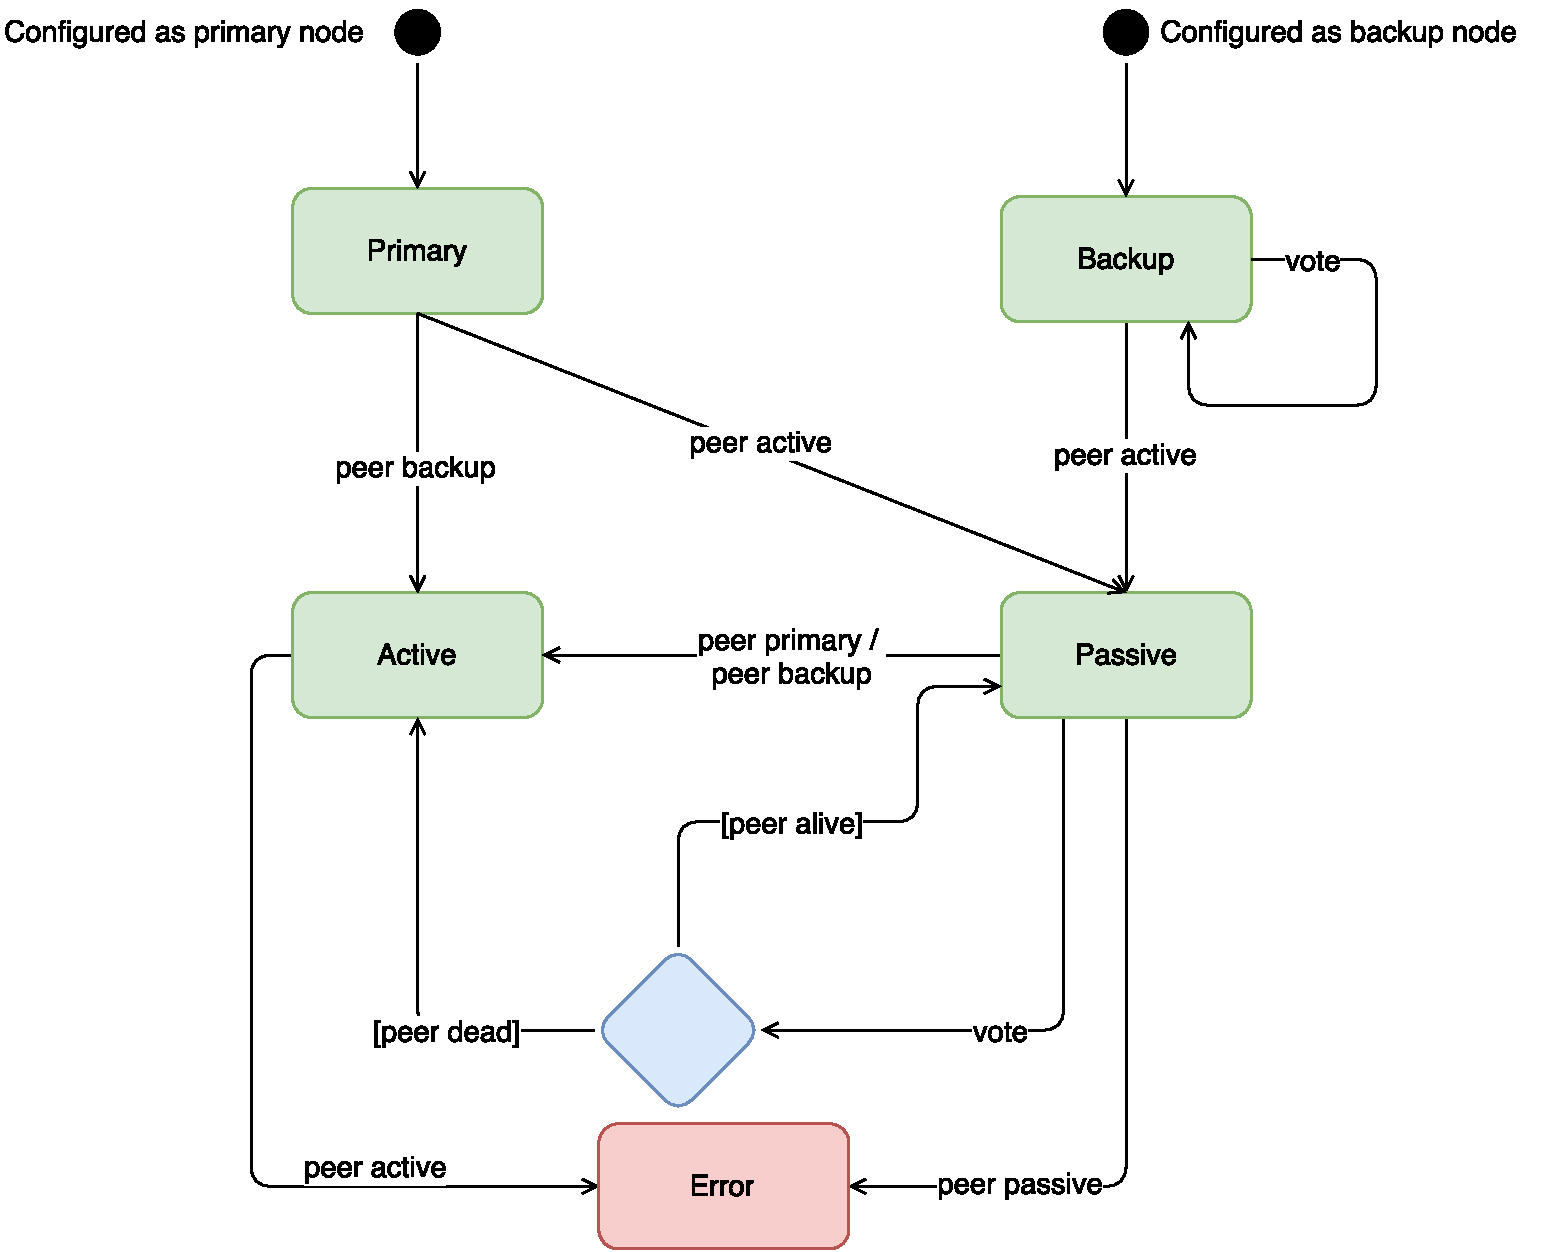
\includegraphics[width=\textwidth]{img/state_machine_diagram_bstar.pdf}
	\caption{BStar machine state diagram}
	\label{fig:bstar:state}
\end{figure}

\subsubsection{Socket types}
The sockets used by both HA peers to send and receive state
updates is a PUB-SUB pair each. Using PUB-SUB sockets makes sense to avoid queues filling up
in case of an actual failure, which PUSH-PULL sockets would do. PUB sockets simply drop messages when there are
no SUB sockets connected, which is the desired effect.


\subsubsection{Configuration}
The DSL has been extended to support an additional property called
\sh{backup_endpoints}. Furthermore, the hashmaps stored in the properties for
the primary and backup endpoints simply contain another endpoint each: The ones
used by the COMM.BSTAR actors. This is illustrated in \autoref{lst:dsl:topo:with-ha}.
Using this information, direct subnodes of a HA node can determine the correct
supernode, as well as know the other node's endpoints in case the currently
active HA peer fails.



\begin{listing}
	\begin{minted}[bgcolor=bg]{Ruby}
module Conf::Federation
  def self.conf
    proc do
      primary_endpoints \
        router: 'tcp://0.0.0.0:20000',
        pull:   'tcp://0.0.0.0:20001',
        pub:    'tcp://0.0.0.0:20002',
        ha_pub: 'tcp://0.0.0.0:20003'

      backup_endpoints \
        router: 'tcp://0.0.0.0:20010',
        pull:   'tcp://0.0.0.0:20011',
        pub:    'tcp://0.0.0.0:20012',
        ha_pub: 'tcp://0.0.0.0:20013'

      adapters do
        # telnet server for client systems (fake OPC-UA HA interface)
        adapter :telnet do
          label           'Telnet'
          desc            'Telnet Server'
          adapter_class   Roadster::Adapters::TelnetServer

          peer :server do
            label   'LTA'
            desc    'LTA'
            uri     "tcp://0.0.0.0:#{Roadster.conf.telnet_server_port}"
          end
        end
      end

      node :s1 do
        # [...]
      end
    end
  end
end
	\end{minted}
	\caption{Federation DSL example with HA.}
	\label{lst:dsl:topo:with-ha}
\end{listing}



\subsubsection{OPC UA}
One of the non-functional goals demanded the HA solution be developed with
\gls{opc-ua} in mind. OPC-UA describes several ways of non-transparent server
redundancy, which seems to map closely to how the \gls{bstar} works.

\subsubsection{State machine}
A finite state machine comprises the core of the \gls{bstar}. It is implemented
as a private method \mintinline[bgcolor=bg]{Text};#fsm; which does nothing but
state transitions based on the current state and a trigger event.
\autoref{lst:approach:bstar:fsm_1} and \autoref{lst:approach:bstar:fsm_2}
illustrate the complete method.

The actual states and events are \sh{Symbol}s registered as
constants in the modules
\begin{itemize}
	\item \sh{Roadster::Engines::BStar::States} and
	\item \sh{Roadster::Engines::BStar::Events}
\end{itemize}
The first module is illustrated in \autoref{lst:approach:bstar:states}.
This is a good practice because manually
retyping every Symbol such as \rb{:active}, \rb{:passive}, \rb{:client_vote},
etc. is prone to errors. Ruby cannot recognize typing mistakes in Symbol
literals, but it can do so for constants.

\begin{listing}[H]
  \begin{minted}[bgcolor=bg]{Ruby}
      # The states a BStar peer can be in.
      #
      module States
        PRIMARY = :primary # peer is the designated primary peer
        BACKUP  = :backup  # peer is the designated backup peer

        # possible initial states
        INITIAL = [ PRIMARY, BACKUP ].freeze

        ACTIVE  = :active  # peer is currently active
        PASSIVE = :passive # peer is currently passive

        # an array of all possible states
        ALL = [ PRIMARY, BACKUP, ACTIVE, PASSIVE ].freeze
      end
  \end{minted}
	\caption{The BSTAR actor's state.}
  \label{lst:approach:bstar:states}
\end{listing}

\begin{listing}[H]
  \begin{minted}[bgcolor=bg]{Ruby}
# Processes an event using a finite state machine.
#
# @param event [Symbol] the event to process
# @see Events
# @return [void]
# @raise [NotActive] if client request can't be processed because this
#   peer either still in {States::PRIMARY}, {States::BACKUP} or is in
#   {States::PASSIVE} and peer still seems alive
# @raise [SplitBrain] if this peer is {States::ACTIVE} and the other peer
#   reported {States::ACTIVE} as well
# @raise [DualPassives] if this peer is {States::PASSIVE} and the other
#   peer reported {States::PASSIVE} as well
# @return [void]
#
def fsm(event)
  log.debug "processing event #{event.inspect} ..."
  case @state
  when States::PRIMARY
    case event
    when Events::PEER_PRIMARY
      fail UserError, 'Invalid config: double primary'
    when Events::PEER_BACKUP
      log.info 'connected to backup (passive), ready active'
      app_active!
    when Events::PEER_ACTIVE
      log.info 'connected to backup (active), ready passive'
      app_passive!
    when Events::CLIENT_VOTE
      # NOTE: Not going active immediately here because backup node could
      # currently be active.

      if peer_expired?
        # Backup peer seems offline, switch to the active state and
        # accept client connections
        log.warn 'I: backup seems dead, going ready active'
        app_active!
      else
        # If peer is alive, reject connections
        fail NotActive
      end
    end

  when States::BACKUP
    case event
    when Events::PEER_BACKUP
      fail UserError, 'Invalid config: double backup'
    when Events::PEER_ACTIVE
      log.info 'connected to primary (active), ready passive'
      app_passive!
    when Events::CLIENT_VOTE
      # Reject client connections when acting as backup
      fail NotActive
    end
  \end{minted}
	\caption{The BSTAR actor's finite state machine (part 1/2).}
  \label{lst:approach:bstar:fsm_1}
\end{listing}

\begin{listing}[H]
  \begin{minted}[bgcolor=bg]{Ruby}
        when States::ACTIVE
          case event
          when Events::PEER_ACTIVE
            # Two actives would mean split-brain
            log.error 'fatal error - dual actives, aborting'
            fail SplitBrain
          end

        when States::PASSIVE
          case event
          when Events::PEER_PRIMARY
            # Peer is restarting - become active, peer will go passive
            log.warn 'primary (passive) is restarting, ready active'
            app_active!

          when Events::PEER_BACKUP
            # Peer is restarting - become active, peer will go passive
            log.warn 'backup (passive) is restarting, ready active'
            app_active!

          when Events::PEER_PASSIVE
            # Two passives would mean cluster would be non-responsive
            log.error 'fatal error - dual passives, aborting'
            fail DualPassives

          when Events::CLIENT_VOTE
            # Peer becomes active if timeout has passed
            # It's the client request that triggers the failover
            if peer_expired?

              # OPTIMIZE: Only go active with enough votes

              # If peer is dead, switch to the active state
              log.warn 'failover successful, ready active'
              app_active!
            else
              # If peer is alive, reject connections
              fail NotActive
            end
          end
        end
      end
  \end{minted}
	\caption{The BSTAR actor's finite state machine (part 2/2).}
  \label{lst:approach:bstar:fsm_2}
\end{listing}


\subsection{Operation modes}
The concrete difference between an active and a passive HA peer is the mode its
engines are running in. During the initialization process, every engine on a HA
node waits for the signal from the COMM.BSTAR actor to either go active, or go
passive. Having passive as an explicit mode is required, because
the COMM.DOWNSTREAM actually has to register inter-node sockets
correctly, even when passive. This is to ensure that subnodes can send their
votes, as well as domain model updates from the active HA peer can be received and
processed on the passive one.

During the initialization of every engine on a HA node, the engine actually
waits for the signal from the COMM.BSTAR actor to either go active or passive.
To do so, the existing \gls{ACP} has been extended by two message types:
\begin{itemize}
	\item \sh{Roadster::Messaging::ACP::Messages::GoActive}
	\item \sh{Roadster::Messaging::ACP::Messages::GoPassive}
\end{itemize}

These are sent to the CORE actor, which then publishes them to all local actors
via its intra-node PUB socket.

\subsubsection{Going active}
All engines on a non-HA node immediately go active. Engines on the active peer
of a HA node go active right after they get the signal from the COMM.BSTAR
actor.

Going active encompasses the following actions, grouped by actor:
\begin{itemize}
	\item CORE:
		\begin{itemize}
			\item Enable \emph{guard} and \emph{aggregate} evaluations
		\end{itemize}
	\item COMM.DOWNSTREAM:
		\begin{itemize}
			\item Enable publishment of model updates via the PUB socket facing subnodes
			\item Enable pinging of subnodes
			\item Enable replication of persisted data
		\end{itemize}
	\item COMM.UPSTREAM:
		\begin{itemize}
			\item Enable pushing of model udpates to the supernode via the PUSH socket
		\end{itemize}
	\item COMM.*:
		\begin{itemize}
			\item Establish connections with field devices (\emph{adapter peers})
		\end{itemize}
\end{itemize}


\subsubsection{Going passive}\label{sec:approach:ha:going-passive}
This can only happen at the initialization of a Roadster instance. There is no
use of going passive at any later point.

The only action actually taken when
going passive is inside the COMM.DOWNSTREAM actor: Inter-node sockets for
communication with the active HA peer and subnodes have to be registered.

The passive HA peer does not actually ping subnodes. Doing so would require the
subnodes' COMM.UPSTREAM actor's inter-node sockets to connect to multiple
endpoints. While possible with DEALER sockets, messages would get sent to the
remote sockets in round-robin mode. A deterministic message passing to one of
the two supernodes (active and passive) is not possible. ROUTER-ROUTER
communication and prepending the correct \emph{envelope} would be required for
this. But there's really no benefit in pinging subnodes from more than one
supernode.


\subsection{Failover}
The passive HA peer takes over when the following two conditions are met:

\begin{enumerate}
\item Active HA peer is unresponsive
\item Connection requests from clients
\end{enumerate}

The second condition is to prevent the split-brain syndrome and thus can be
thought of as an external vote for the node to actually initiate the failover.
This works because clients will try to (re-)connect to the HA peers in
round-robin fashion.  This algorithm is explained in \cite[Chapter 4 - Reliable
Request-Reply Patterns, Client-Side Reliability (Lazy Pirate
Pattern)]{zmq:zguide}.

In case the currently active peer crashes, the two conditions will be met.
This means that the COMM.BSTAR actor on the passive HA peer tells all other
engines to go active using the designated new \gls{ACP} message type.


\subsubsection{No vote, no failover}
A failover can only happen if there is at least one vote. With a total absence
of subnodes and client systems, a failover cannot happen. Thinking about it, it
is not a bad thing if the failover cannot happen in that case, since there is
no client depending on the service brought by a HA cluster.

\subsubsection{Alarm generation}
When a failover happens, it makes sense to create an alarm case
so the outage is visible to operational personnel in one of the web UIs.

% TODO using Guard + proof reading
To generate an alarm case it is possible to set a guard which observes
a variable in the DIM and when the variable changes and the appropriate 
condition is met the guard will automatically generate a defined alarm case.
Only core actors can have guard, the feature is disabled on the ohter actors,
therefore it is important to publish the DIM update to the core otherwise
it will never generate an alarm case.

The same applies to the case where the passive HA peer fails, although it
does not have an immediate effect on availability.  This is so the operational
personnel can act upon the alarm and e.g. initiate field forces to inspect the
failed node and repair it.

Once repaired, it is restarted with the exact same configuration --- either primary
or backup. Since there is already an active HA peer (either the primary one,
or the backup one), the newly repaired node will become the new passive HA peer.

\subsubsection{Failover from backup to primary node}
Once failed over, the newly active backup node stays active. It does so until it
fails itself or is manually stopped. It never automatically switches back to
make the primary node the new active one without a failure. This is key. If a
node becomes unreachable, the failover happens automatically, but anything else will
require human interaction.

Subsequently, when the previously broken, primary node has been repaired, it
rejoins the \gls{bstar} cluster as the passive HA peer. At that point, the backup
node can be killed if need be, and the primary node will take over again.  This
works because the \gls{bstar} operates symmetrically after a successful
handshake during initialization.

\subsection{Replication}
% diagonal HA
The passive HA peer needs to stay up-to-date, i.e. subscribe to model updates
affecting the DIM as well as updates to persisted data.
Instead of clients replicating modifications to both HA peers, as
described in \cite[Chapter 5 - Advanced Pub-Sub Patterns, The Clustered Hashmap
Protocol]{zmq:zguide}, the passive HA peer could just act as a supernode of the
active HA peer. This eliminates the need for an additional protocol. In case of
a failover, the roles of course need to be exchanged.

% TODO: what if HA cluster has supernode
A problem arises if the HA cluster has a supernode (although
considered an unusual case). That would mean the active peer has two supernodes
connected at the same time, which is not supported by the planned communication
infrastructure. One solution would be to use a ROUTER socket in the
COMM.UPSTREAM actor as well, to be able to decide which of the two supernodes
is the actual receiver of a message. This idea has already been mentioned in
\autoref{sec:approach:ha:going-passive}.

A different, and simpler solution would be to perform the
replication to the HA peer only via sockets of the two BSTAR actors. This would
actually allow reducing the complexity in the COMM.UPSTREAM and COMM.DOWNSTREAM
actors, because they would not have to take part in any communication with the
other HA peer. This is described as a refactoring opportunity in
\autoref{sec:disc:ha}.

\subsection{A note on dedicated links}
The \gls{zguide} mentions that a dedicated network link between the two HA peers
(traditionally done with a crossover cable) is the best solution to prevent the
split-brain syndrome. This is true. But in some cases, it could also prevent a
failover from happening.

Supposing that part of the currently active peer's network equipment fails, i.e. one
of its \glspl{NIC} connected to the switch fails, or one of its switch ports
fail. In that case it will be unreachable to the rest of the
federation or to the client system. A failover would be desired. But a failover
cannot be initiated, since heartbeats will still be exchanged with the passive HA peer over
the dedicated link. So it is a trade-off between risking the split-brain
syndrome and not being able to perform a failover.

\subsubsection{Extending the \gls{bstar}}\label{sec:approach:ha:bstar-ext}
% vision
Of course the \gls{bstar} mechanism could be extended to handle cases where the
active peer loses connectivity to its subnodes, but not to the other HA peer. In
a situation like that, the passive HA peer could actually take over to minimize
service downtime. The active HA peer could communicate the number of fully connected subnodes,
which would be zero in case of a network partition. That way, the
passive HA peer could recognize the situation correctly, since it will receive
requests from subnodes, which are trying to fallback to the passive HA peer since
the active HA peer is unresponsive. Knowing that the active HA peer has zero
connected subnodes, it could promote itself to the new active HA peer and
communicate this to the other HA peer.

% what's needed for higher-level clients
\paragraph{Client systems}
For this to work, a way of counting fully connected (not just requesting)
and client systems would have to be introduced. The COMM actor providing the \gls{opc-ua}
interface would know best how many clients are connected. This would solve the problem for single-level HA setups.

% what's needed for subnodes as clients
\paragraph{Subnodes}
In case of a multi-level federation with a HA cluster at its root. Because nodes within a
federation communicate with each other via \zmq sockets, telling how many
clients are connected is not straight-forward, because \zmq abstracts
connection handling completely away. The \gls{zguide} declares such needs as application matter.
The subnodes would have to implement application-level heartbeating.
That is, the subnodes that are fully connected at a given point in time (i.e. enrolled
in the DIM replication) would periodically send heartbeats which could then be
used to maintain an up-to-date list of active clients (where stale client
entries automatically expire).  The number of active clients (the size of the
list) could be communicated privately just between the two HA peers, along with
the heartbeats. Publishing that information via the DIM might be problematic,
since DIM updates go over the main network link.

% step down from active to passive
\paragraph{Stepping down}
Something else needed is a HA peer's ability to step down from being the
active HA peer as soon as its peer promotes itself to the newly active peer. In
the standard \gls{bstar} mechanism, this would be recognized as the split-brain
syndrome and handled fatally.

% discard because KISS
\paragraph{KISS}
Doing this without an actual need would be a violation of the \gls{KISS} principle,
so the first approach will not include any extensions to the \gls{bstar}.

\subsubsection{Corner case}
A highly unlikely, but dangerous corner case \emph{could} lead to the
split-brain syndrome. The following steps would be required to happen:

\begin{enumerate}
	\item The backup node is currently the active one

	\item Then the dedicated link fails, which means no heartbeats are
		exchanged anymore

	\item A new client tries to connect or an existing one is temporarily
		gone and tries to reconnect
\end{enumerate}

Since clients try to contact the primary node first, this could
lead to dreaded the split-brain syndrome. The primary node does not hear any
life signs from the backup node (the rightfully active peer), and client
requests count as votes. This means it will promote itself to the active peer,
even though the backup node is still active.

\subsection{A note on heart beating}\label{sec:approach:ha:hb}
Special attention needs to be paid when it comes to sending heartbeats within a
HA cluster. A na\"ive developer might implement the COMM.BSTAR actor so it
autonomously sends heartbeats. This works as long as the failures only affect
the hardware. But what if a software error happens in the CORE actor?  A
Roadster node certainly cannot function without the CORE actor. In that case the
BSTAR actor should not send out heartbeats anymore.

A better implementation would have the BSTAR actor periodically inquire (PING
request) the CORE actor whether it is still healthy, and only send out a
heartbeat in case it gets a response (PONG) in time. This can be done with a
simple mechanism, where the CORE actor is programmed to respond to every PING
request with a PONG response. Similar infrastructure of Roadster could be used
instead, if it already provides it.

Further ideas based on this fundamental mechanism are discussed in
\autoref{sec:discussion:imp:ha:hb}.

%----------------------------------------------------------------------------
\section{Persistence synchronization}\label{sec:approach:psync}
% TODO: big picture - not necessary
The persisted data and updates to it, handled by the STORAGE actor, need to
be replicated up in the topology and collected in the root node.

There are multiple aspects involved in persistence synchronization:

\begin{description}
	\item [Event journal:]\hfill\\

		Event journal data is not
		append-only. Existing cases can still be modified, e.g. to
		confirm them. So the solution to get the full delta of
		modifications, but not more than needed, is to request the
		oldest non-finished case for each owning subnode (direct and
		indirect ones).

	\item [Time series:]\hfill\\
		The good thing about time series is
		that the records, once written, will not be modified. That allows
		for a very simple method of getting new time series records by
		just requesting all records added after a particular point in
		time, per series. However, since old time series data is
		deleted after a certain amount of time (e.g. 6 months), the
		timestamp of oldest record remaining also needs to be requested
		by the supernode, per series, so it can delete them from its
		local files as well.

	\item [Parameters:]\hfill\\
		Every parameter is owned by a node, and is
		synchronized through the DIM.  What is persisted is merely the
		last updated value so the node is able to boot with not only
		sensible defaults, but actual values that are most likely still
		correct.
\end{description}


\subsection{Variants}
There are multiple variants to achieve the needed functionality.

\subsubsection{Polling only}
The supernode just periodically request persistence
deltas. This would be handled over a DEALER-ROUTER pair of sockets. The nice
thing about this variant is that the subnode only has to do one thing, which is
responding to requests from the supernode(s); it does not have to proactively
send any updates after sending the an initial delta.

A big drawback is that the synchronization only happens periodically. This
does not seem to fit well into the overall Roadster architecture, which is
completely event-driven (no polls or "sleeps").

Another drawback is efficiency. This variant will periodically cause the
subnode's database to be searched for possibly large amounts of keys. Depending on the size of the
database and the efficiency of searching through keys, this could be a lot of
wasted resources or even cause bottle necks when interacting with the STOR
actor.

Overall, this variant is very simple, but does not offer some features we'd
normally expect from a framework like Roadster. The fruits are hanging low;
achieving event-driven synchronization and better efficiency is easy.

\subsubsection{Event-driven}
This variant would avoid the delays introduced by the polling mechanism of the first
variant. Just like with the \gls{CSP}, the initial delta is requested and
communicated via the ROUTER-DEALER pair. As soon as the transmission of the
delta begins, the subnode also starts propagating any new modifications via the
PUSH socket. The supernode collects modifications from all subnodes through its
PULL socket.

To avoid filling the PUSH socket unnecessarily in case the supernode is
temporarily unavailable, the heartbeating done via the COMM.UPSTREAM and COMM.DOWNSTREAM actors will
be used to recognize such a situation. The continuous propagation of
modifications can be stopped, the sockets reinitialized, making the node ready
for whenever the supernode is back available.

\subsection{Chosen Variant}
We have chosen the polling variant because our client favored this variant and
it is the simplest solution to implement.  Subnodes do not need extra logic for
the case that a supernode is unreachable.  It is the supernode's responsibility
alone to request deltas of persisted data.


\clearpage
\section{Encryption}\label{sec:approach:encryption}
It is fairly easy to enable transport security to secure the communication
on inter-node \zmq sockets over an insecure network.

\subsection{Assigning socket roles}
Regarding the CURVE security mechanism in \zmq, one of the two involved sockets
needs to be designated as the CURVE server, and the other one as a CURVE
client. This will be done intuitively: A supernode's
COMM.DOWNSTREAM actor's sockets will act as CURVE servers, and a subnode's
COMM.UPSTREAM actor's sockets will act as CURVE clients. This is not just an
arbitrary choice: A CURVE client socket is given exactly one CURVE server
certificate. A supernode can have multiple subnodes, but the opposite is
impossible. Thus, the socket registered by the supernode's
COMM.DOWNSTREAM actor will be designated as the CURVE server, and the sockets
registered by the subnodes' COMM.DOWNSTREAM actors will be designated as CURVE
clients. An example of the client side is shown in \autoref{lst:auth:fednf}, as
performed by the COMM.UPSTREAM actor.

\begin{listing}
	\inputminted[bgcolor=bg]{Ruby}{listings/auth/fednf.rb}
	\caption{Example: Enabling CURVE mechanism on the client.}
	\label{lst:auth:fednf}
\end{listing}

\subsection{Key distribution}
% keys on both sides, and which nodes need whose public key
In addition to the server authentication, which is always performed, client
authentification is desired. This means that each federation node must be
in possession of its respective subnodes' public keys as well (not only the
respective supernode's public key).

% distribution of public keys
Public keys and the private keys are generated in pairs.  Due to
the nature of public keys, they can be distributed conveniently and safely
through the shared configuration file that defines the federation
topology. Curve25519 keys are 256 bits long, which results in only 40 ASCII
characters in \gls{Z85} notation.

% distribution of secret keys via SSH
However, distributing the private keys is less convenient, since they must be kept
private. This can be done via \gls{SSH}, logging into each node and generating
the key pair right on the node itself. This way, the private keys would never
even touch the network. The \sh{roadster} command has been extended with a new
subcommand \sh{keygen} to automate this process. It is passed the node-specific
configuration file, which points to a private key file. A new, securely
generated private key is created at that file location, and the associated
public key is printed on the terminal. Automating the storage of the private
key in the correct file is not only a convenience, but also helps security: If
printed on the terminal, it could linger around somewhere in the terminal
scrollback buffer, or go unnoticed in the clipboard, in the shell history, etc.

Given that Roadster is only a framework, there will be a Git repository
containing the specifics of a given Roadster installation, just like the
example application provided by mindclue GmbH for this bachelor thesis.
This fact is very useful when it comes to the distribution of public keys.
The following procedure can be followed to generate the required keys in
advance and make them available through the shared configuration:

\begin{enumerate}
	\item for all nodes
	\begin{enumerate}
		\item SSH into the node
		\item Pull new commits from the central repository
		\item Generate key pair on the node itself using the \sh{roadster keygen} utility
		\item Put the public key into the shared configuration
		\item Commit the modified configuration, and push it back to a central repository
	\end{enumerate}
\end{enumerate}

This procedure could be implemented as a script that performs the procedure
over \gls{SSH} while the nodes are still in the
lab (assuming that is secure). Of course that script could also be used when
the nodes are already installed in a production environment. However, for that to be
secure, the nodes' authenticity must have been verified in advance. Otherwise,
man-in-the-middle attacks would be possible while logging into the nodes,
compromising everything.

\subsubsection{ZAP}
A socket designated as CURVE server needs a way to authenticate arriving client
connections. This is done via an in-process \gls{ZAP} authentication handler,
as described in \autoref{sec:zmq:security}. That authentication handler
needs to be able to access all clients' public keys to be able to perform its
job.

The ZAP protocol (used between a CURVE server socket and the authentication
handler) is very simple and thus makes it possible to relay the authentication
requests from there to a central ZAP authentication handler, so all clients'
public keys could be stored and managed centrally. But that would violate the
autonomy requirement, so this idea has been discarded immediately.

CZMQ provides an authentication handler\footnote{It is simply a function
(\cpp{zauth()}) that is executed by a CZMQ actor. The whole construct is
abstracted in CZTop through \rb{CZTop::Authenticator}.} that can lookup public
keys awaiting authentication in a designated directory on the file system,
which it does by instantiating a certificate store.\footnote{That certificate
store is a class in CZMQ called \cpp{zcertstore}, represented through
\rb{CZTop::CertStore} in CZTop.} The certificate store in turn looks up the
certificates on disk by the public key in question.

There is also the possibility of providing an already instanciated certificate
store to the authentication handler. This is useful because a certificate store
allows the insertion of certificates (public keys) in-memory, avoiding the need
to load certificates from disk. This greatly simplifies the key distribution.
Public key files will not have to be copied from one node to its subnodes
anymore. Instead, they can be taken directly from the shared configuration file
that defines the federation topology. As an example, \autoref{lst:auth:fedsf}
shows how to start an authentication handler which does client authentication
as it is done inside the DOWNSTREAM actor.

\begin{listing}
	\inputminted[bgcolor=bg]{Ruby}{listings/auth/fedsf.rb}
	\caption{Example: Enabling CURVE mechanism including client authentication.}
	\label{lst:auth:fedsf}
\end{listing}

\paragraph{Failover}\label{sec:approach:encryption:ha}
It is possible that a node's supernode is actually a HA cluster consisting of
two nodes. Those two nodes should have their own key pairs for additional
security. This imposes a problem for the subnodes: It is only possible to assign
a single CURVE server public key. In case the active HA peer becomes
unresponsive and the subnode(s) falls back to the passive HA peer, a new CURVE
server public key needs to be assigned to the client sockets. This should be
possible. But there's a better solution:
Since the socket could be \cite[Binary Star Implementation, Binary Star client
in C]{zmq:zguide} ``confused''\footnote{This probably applies only to REQ
sockets, since they implement \cite[Client-Side Reliability (Lazy Pirate
Pattern)]{zmq:zguide} ``a small finite-state machine to enforce the
send/receive ping-pong''}, it is good practice to simply destroy the existing
socket and create a fresh one, assigning the correct supernode's CURVE server
certificate to it.

\paragraph{IP based access control}
In addition to the CURVE mechanism, blacklisting or whitelisting clients based
on their \gls{IP} addresses is possible and supported by
\rb{CZTop::Authenticator} through the PLAIN mechanism. It would even be
feasible to whitelist the exact client IP addresses, since they can be deduced
from the shared configuration. But it is not part of requirements and thus will not
be done within the scope of this bachelor thesis.


\subsection{End-to-end security}
Encrypting and authenticating network traffic is good, but it only secures the
communication between two neighboring nodes. Messages could travel via multiple
hops to reach their destination node. To provide end-to-end security for such
messages, they need to be authenticated as well, using cryptographic
signatures.

The challenge here is to decide on what to sign. Ruby objects are serialized
into \glspl{BLOB}, which is perfectly suitable as input for a \gls{MAC} algorithm.
This is possible because the message's on-wire
representation doesn't change from origin to destination.

The codecs implemented in Roadster, which serialize a message into the an
on-wire representation, are part of the messaging layer. This fact makes it
hard to adapt the existing codecs to add authentication. The codecs should be
the final authority before the message is sent via a socket, and should be the
first to inspect an arriving message. The advantage is that a forged,
unauthentic message can (and must) be discarded immediately, without even
decoding it.  Because Ruby marshalling allows the serialization and
deserialization of almost any object, merely decoding a message could be
dangerous, as described by the Ruby documentation itself on \cite[Security
considerations]{rb:doc:marshal}.  For this reason, the codecs need to be moved
from the messaging layer down to the reactor layer.


\subsubsection{Implementation}
The codecs have been adapted to sign \emph{tag} and authenticate messages using
an authenticator object, an instance of the
new class\\\sh{Roadster::Actors::MessageAuthenticator}. It offers the two
instance methods \mintinline[bgcolor=bg]{Text};#tag; and \mintinline[bgcolor=bg]{Text};#authenticate!;.
Codecs --- which are stateless, only offering \sh{.encode} and \sh{.decode}
class methods --- are passed the authenticator object.

The resulting MAC \emph{security tag} is stored in an additional \zmq frame
before the message BLOB itself. Thus, the codec version (sent in the first
frame of every message) has been updated to represent the incompatible change.
It is important that the new frame is only used as a MAC and not any other
information, as the authenticity of any other information cannot be verified.

Intra-node messages do not have to be authenticated, whereas inter-node
messages have to be. This requires some logic to be present in the codecs
to only use the authenticator on inter-node sockets. To reduce
code complexity, and also because codecs have no knowledge about sockets, the
\emph{Null Object} design pattern has been used. When a socket is passed a
message to be sent, or when receiving a message, the appropriate authenticator
object is passed, which is either an instance of
\sh{Roadster::Actors::MessageAuthenticator} for inter-node sockets, or
\sh{Roadster::Actors::MessageAuthenticator::Null} for intra-node sockets.


\section{OPC UA Interface: High availability}\label{sec:approach:opc-ua}
Some client systems interact with Roadster over the standardized \gls{opc-ua}
interface. According to the standard in \cite[6.4.2 Server Redundancy,
p.~94]{opc-ua:behavior:server-redundancy}, there are multiple ways to ensure
interoperability when running the root node as a \gls{HA} cluster. The variant
which comes closest to the \gls{HA} mechanism favored in the original task description is
\emph{Non-transparent server Redundancy}, where the client system is aware of
the hot-standby setup. Specifically, it also has to be aware of the failover
mode. Described failover modes in the standard are \emph{Cold}, \emph{Warm},
\emph{Hot} and \emph{HotPlusMirrored}. The mode \emph{Warm} describes the
favored failover mode best, quoting \cite[6.4.2.4.4 Server Failover Modes,
p.~98]{opc-ua:behavior:server-redundancy}:


\begin{quote}
``Warm Failover mode is where the backup Server(s) can be active, but cannot
connect to actual data points (typically, a system where the underlying devices
are limited to a single connection). Underlying devices, such as PLCs, may have
limited resources that permit a single Server connection. Therefore, only a
single Server will be able to consume data. The ServiceLevel Variable defined
in Part 5 indicates the ability of the Server to provide its data to the
Client.''
\end{quote}

The concept to induce a failover in a \gls{HA} cluster (limited to a
Roadster federation only, excluding client systems) as part of the
COMM.UPSTREAM actor's responsibilities can actually be implemented in any other
actor, e.g. an adapter facing client systems. All the adapter on the passive
node has to do is send a vote to the COMM.BSTAR actor in case the client system
tries to connect and request a service. The following code would be sufficient:

\begin{listing}[H]
  \begin{minted}[bgcolor=bg]{Ruby}
msg = Messaging::BSP::Messages::Vote.new 'comm.opcua', 'comm.bstar'
route_message msg
  \end{minted}
  \caption{OPC-UA adapter: How to send a vote to the BSTAR actor.}
  \label{lst:approach:opc-ua}
\end{listing}

mindclue GmbH actually offers an adapter implementing the \gls{opc-ua}
interface, wrapped into a Ruby software package. Unfortunately, an
incompatibility in the package's dependencies, makes its use impossible at the
moment. Instead, an implementation of a simple Telnet server is planned. The
server shall recognize the command \sh{VOTE!}, and perform the required steps to
relay the vote to the COMM.BSTAR actor.
